\documentclass[3p]{elsarticle}

\makeatletter
\def\@author#1{\g@addto@macro\elsauthors{\normalsize%
    \def\baselinestretch{1}%
    \upshape\authorsep#1\unskip\textsuperscript{%
      \ifx\@fnmark\@empty\else\unskip\sep\@fnmark\let\sep=,\fi
      \ifx\@corref\@empty\else\unskip\sep\@corref\let\sep=,\fi
      }%
    \def\authorsep{\unskip,\space}%
    \global\let\@fnmark\@empty
    \global\let\@corref\@empty  %% Added
    \global\let\sep\@empty}%
    \@eadauthor={#1}
}
\makeatother

\usepackage{lineno}
\usepackage{color}
\usepackage[hidelinks]{hyperref}
\usepackage{graphicx}
\usepackage{caption}
\usepackage{epstopdf}
\usepackage{multirow}
\usepackage{lineno}
\usepackage{amssymb}
\usepackage{pgfplots}
\usepackage{tikz}
\usepackage{subcaption}
\usepackage{rotating}
\usepackage{threeparttable}
\usepackage{setspace}
\usepackage{flexisym}
\usetikzlibrary{matrix}
\usetikzlibrary{spy}
\usepgfplotslibrary{groupplots}
\pgfplotsset{compat=newest}
\graphicspath{ {./figures/} }



\modulolinenumbers[5]
\journal{Journal of \LaTeX\ Templates}

%%%%%%%%%%%%%%%%%%%%%%%
%% Elsevier bibliography styles
%%%%%%%%%%%%%%%%%%%%%%%
%% To change the style, put a % in front of the second line of the current style and
%% remove the % from the second line of the style you would like to use.
%%%%%%%%%%%%%%%%%%%%%%%

%% Numbered
%\bibliographystyle{model1-num-names}

%% Numbered without titles
%\bibliographystyle{model1a-num-names}

%% Harvard
%\bibliographystyle{model2-names.bst}\biboptions{authoryear}

%% Vancouver numbered
%\usepackage{numcompress}\bibliographystyle{model3-num-names}

%% Vancouver name/year
%\usepackage{numcompress}\bibliographystyle{model4-names}\biboptions{authoryear}

%% APA style
%\bibliographystyle{model5-names}\biboptions{authoryear}

%% AMA style
%\usepackage{numcompress}\bibliographystyle{model6-num-names}

%% `Elsevier LaTeX' style
\bibliographystyle{elsarticle-num}
%%%%%%%%%%%%%%%%%%%%%%%

\begin{document}
\doublespacing
%\Large
%\setstretch{1.1}


\begin{frontmatter}

\title{Effects of barrelling formation during the axial compressive tests of cubic
samples with  isotropic, transversely isotropic and orthotropic elastic
properties} 

%%\tnotetext[mytitlenote]{Fully documented templates are available in the
% elsarticle package on \href{http://www.ctan.org/tex-archive/macros/latex/contrib/elsarticle}{CTAN}.}

%% Group authors per affiliation:






%%\fntext[fn1]{This is the specimen author footnote.}
%%\fntext[fn2]{Another author footnote, but a little more longer.}
%%\fntext[fn3]{Yet another author footnote. Indeed, you can have any number of
% author footnotes.}
\cortext[cor1]{Corresponding author}
\author{Alexey Vorobyev\corref{cor1}}
\ead{alexey.vorobyev@me.com}


\author{Ingela Bjurhager}
\author{Nico P. van Dijk}
\author{Kristofer Gamstedt}

\address{Division of Appplied Mechanics, Uppsala University, Box 534,
SE-751 21, Uppsala, Sweden}



\begin{abstract}
For scarce materials, such as archaeological wood, one often resorts to cubic
samples instead of standardised prisms for mechanical tests, since the elasticity can be tested in all three direction in one sample. For such samples
barrelling  formation gives rise to additional difficulties difficulties in
identifying the elastic properties.
Furthermore natural orthotropy, availability and variation between and within
samples make the mechanical characterisation of wood  challenging. 
The purpose of the present study is numerically investigate the effects of barrelling
in cubic samples during compressive experiments. Secondly, to investigate and
compare barrelling formation on isotropic, transversely 
isotropic and orthotropic material parameters. 
Finally to compare four strain measurement techniques using
digital image correlation , strain gauges and direct
reading from the testing machine and investigate which is better for
quantification of mechanical parameters such as Young's moduli and Poisson's ratios.
The elastic parameters determined from the simulated tests were normalised with regards to the input parameters. The presented relative errors provide information when the perturbation caused by barrelling effect is negligible or significant for various materials and strain measurements. 
As an example, compressive tests on waterlogged archaeological oak impregnated
with polyethylene glycol are discussed.



\end{abstract}

\begin{keyword}
Cubic samples\sep Compressive testing\sep Barrelling formation \sep
Wood
\end{keyword}

\end{frontmatter}

\linenumbers

\section{Introduction}

Characterisation of material stiffness properties of orthotropic materials can
be challenging. In  careful design of wood structures, not only one parameter,
but the full orthotropic set of elastic parameters is needed \cite{tsoumis1991science},
e.g. for finite-element modelling of wood joints that are locally subjected to a
triaxial stress state. Compressive experiments are generally considered to be
reliable method for identifying engineering constants such as Young's moduli and Poisson's ratios. The general approach is to measure the material response due to applied
forces. The procedure is straightforward and easy to perform due to simplicity of experimental installation and low requirements to sample
geometry. ASTM D143 standard \cite{standard1997d143,
johnson1983compression} require the usage of elongated rectangular prisms for
the compressive testing along with strain gauges.
For rare materials such as archaeological wood, it is more convenient to use
cubic samples \cite{ljungdahl2007transverse, vorobyevcharacterisation} to save
material.
This enables the same sample to be tested several times and in
different directions (typically radial, tangential, longitudinal) if the loads are
applied within the elastic range and do not cause and irreversible damage in the material.
A disadvantage of compressive testing of cubes compared to the tensile testing
of dog-bone samples is that it can be difficult to ensure a homogeneous stress
state due to geometrical imperfections in the test samples
\cite{Toftegaard1999849}.
Moreover, barrelling  (as illustrated in Figure \ref{fig:barrelling}) during
compressive loading \cite{oldroyd1966stress} caused by friction between the platens and the
sample makes it difficult to assess the non-uniform deformation in order to
determine the elastic parameters.
Consequently, the Poisson's ratios cannot be obtained directly under such constraints. 
The classical way to measure strain is by using the loading platen position or electrical-resistance strain gauges. Nowadays, full field strain measurement techniques such
as digital speckle photography (DSP) \cite{synnergren1999stereoscopic} and
3D/stereo-digital image correlation (DIC) \cite{majano2012test} are 
increasingly being used.The strain-field measurement technique using
DIC has been shown advantages in comparison with the traditional strain gauges
\cite{huang2010optical,xavier2012stereovision}. In particular, full-field measurements can help to improve the estimation of the stiffness parameters \cite{dahl2009planar,
majano2012test, ozyhar2013moisture}. 
Despite technical difficulties in obtaining accurate elastic properties by compressive testing of wooden cubes, it is still a reasonable 
choice of test method if the amount of available material is limited, as is the case for e.g.\ archaeological material. The intention of the present work is to estimate how large the measurement errors can due to the inevitable barrelling effect, and which strain measures are suitable to reduce such errors.  \par 

This study was initiated when in order to better estimate the stiffness properties of water-logged and preservation-treated  oak of the Vasa shipwreck, displayed at a public museum in Stockholm. The stiffness of the material is needed as input parameters in a finite-element model of the ship, which can be used in the design of a future improved support system for the ship. The Vasa capsized in 1628, and was salvaged in 1961. 
The waterlogged ship was impregnated with polyethylene glycol (PEG) in an extensive conservation process aiming to prevent deformation during drying. 
Extensive research during the last decades have shown that the ship is suffering
from aggressive chemical degradation. Both the degradation \cite{bjurhager2012state}
and the PEG impregnation \cite{ljungdahl2007transverse} have had a negative effect on the mechanical properties of the ship, which is in need of a better support. \par
Previously compressive experiments on prismatic samples with orthotropic
material behavior were simulated by Toftegaard \cite{Toftegaard1999849} who investigated the effect of geometrical imperfections on the
engineering elastic constants.
In his work Toftegaard compared the simulated strain field to the measurements
of strain gauges and obtained good agreement between the simulated and experimental
data.\par
In the present work, DSP has been used in order to obtain the experimental
strain field, based on the displacement field over an area rather than locally
at metallic foil pattern of a strain gauge.
Chen \cite{Chen001} simulated the deformation behaviour of samples with geometrical
imperfections supported by a locked hemispherical seat compared to conventional platens. This is useful for rigid platens which cannot adjust to sample geometry to spread the loads more evenly over the contact area.
\par 

%The purpose of experiment



The purpose of the present work is to investigates the occurence of barrelling
 on the accuracy of the obtained elastic properties in three different types of material behaviour, namely isotropic, transversely isotropic and orthotropic elastic properties, in ranges applicable for archeological wood.
Additionally, four strain measuring techniques using DSP (full field and central
area of interest), strain gauges (recommended by the standard 
\cite{standard1997d143, johnson1983compression}) and direct compressive platen
displacement measurement are compared in order to assess the magnitude of the
resulting errors.
The results can help to estimate the induced errors for the alternative strain measurement methods. 
% 
% This enables testing of the same sample several times and in
% different directions (radial, tangential, longitudinal) if the loads are
% applied within the elastic range.
% A disadvantage with compressive testing of cubes compared to tensile testing of
% dog-bone specimens, is that it can be complicated to ensure a homogeneous stress state
% due to geometrical imperfections of test specimens \cite{Toftegaard1999849}.
% Moreover, barrelling formation (Figure \ref{fig:barrelling}) in compressive
% loading \cite{oldroyd1966stress}, due to friction between the platens and the
% sample, makes it difficult to assess the  deformations.
% Consequently, the Poisson's ratios are thus more difficult to obtain directly from this kind
% of loading.
% The conventional way to measure strains is by using the built in measurement
% system or strain gages. Nowadays, full field strain measurement techniques such
% as digital speckle photography (DSP) \cite{synnergren1999stereoscopic} and
% 3D/stereo-digital image correlation (DIC) \cite{majano2012test} are used more
% and more. Strain field measurements technique using DIC has shown a good
% performance in comparison to the traditional strain gauges
% \cite{huang2010optical,xavier2012stereovision} Additionally it helps to
% improve the estimation of the stiffness parameters \cite{dahl2009planar,
% majano2012test, ozyhar2013moisture}. 
% Nevertheless, compressive testing of wooden cubes is the reasonable 
% choice of test method if the amount of available material is limited, as is the case for archaeological material.\par 
% 
% In 2012, a project with the aim of designing a new support structure for the
% archaeological Vasa ship was initiated. The ship was capsized in 1628, and was salvaged in 1961. 
% The waterlogged ship was impregnated with polyethylene glycol (PEG) in an extensive conservation process aiming to prevent deformation during drying. 
% Extensive research during the last decades have found that the ship suffers from
% aggressive chemical degradation. Both the degradation \cite{bjurhager2012state}
% and the PEG impregnation \cite{ljungdahl2007transverse} have had a negative effect on the mechanical properties of the ship, which is in need of a better support. In 2012 a project with the aim of 
% designing a new support structure for the fragile and soft ship was also initiated. For this task, the elastic, ultimate and creep properties of the 
% Vasa oak need to be determined. Due to the limited access to material, cubic samples which can be tested several times is preferred.
% In order to verify the results from the compressive experiments the effect of
% barrelling was investigated by the simulation using the Finite Element
% Modelling (FEM).\\
% Previously compressive experiments on prism samples with orthotropic material
% behavior were simulated by Toftegaard \cite{Toftegaard1999849} in order to
% investigate the effect of geometrical imperfections on identification of
% engineering elastic constants.
% in his work he compared the simulated strain field to the measurements of strain
% gauges and obtained good agreement between the simulated data and experimental
% curves.\par
% The present work uses DSP in order to obtain the experimental strain field,
% based on the displacements in an area rather than two points using a strain
% gauge.
% Chen \cite{Chen001} has simulated the behaviour of specimens with geometrical
% imperfections on a locked  seat during the compressive experiments
% of composite materials. This is relevant when the platens of universal testing
% machine are locked and cannot adjust to sample geometry.
% When a prism specimen is compressed between platens it expand transversely.
% Its surfaces bear heterogeneous deformation that are resulting in barrelling
% formation of the prism.\par 
% 
% % %The purpose of experiment
% 
% 
% 
% The present work investigates
% barrelling formation in three different types of material behaviour.
% Additionally three strain measuring techniques using DSP and strain gauges are
% compared in order to identify the magnitude of resulting errors.
% The results can help to identify the accuracy of the material constants values
% of elastic parameters that can be obtained during compressive experiments on
% cubic samples.


\section{Materials and Methods}

\begin{figure}
    \centering
    \begin{subfigure}[b]{0.4\textwidth}
        \centering
        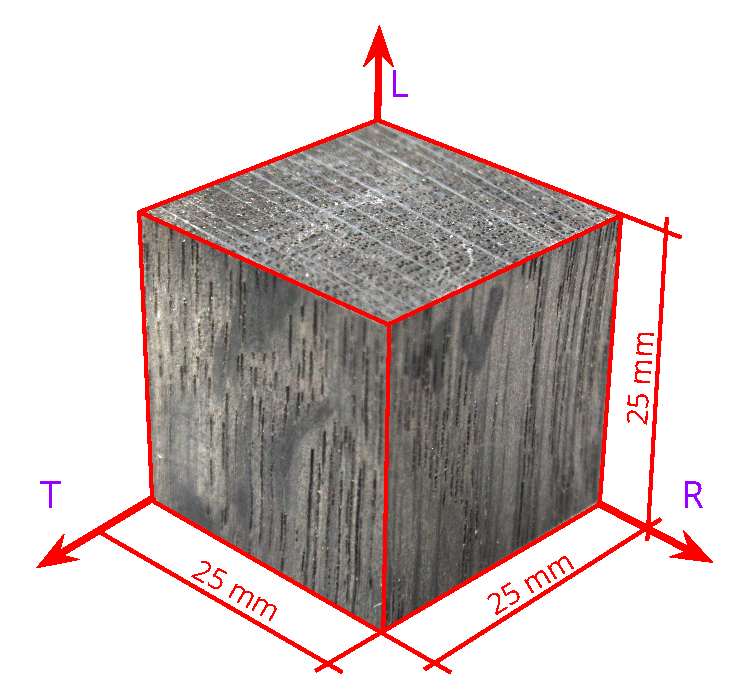
\includegraphics[width=\textwidth]{VasaCube.pdf}
        \caption{}
        \label{fig:vasacube}
         \vspace*{1cm}
    \end{subfigure}
    \hfill
    \begin{subfigure}[b]{0.4\textwidth}
        \centering
        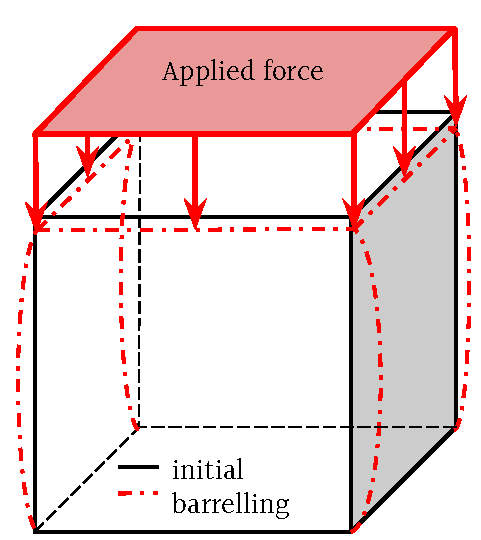
\includegraphics[width=\textwidth]{BarellingEffectZoomed.pdf}
        \caption{}
        \label{fig:barrelling}
        \vspace*{1cm}
        
    \end{subfigure}
    \hfill
    \begin{subfigure}[b]{0.4\textwidth}
        \centering
        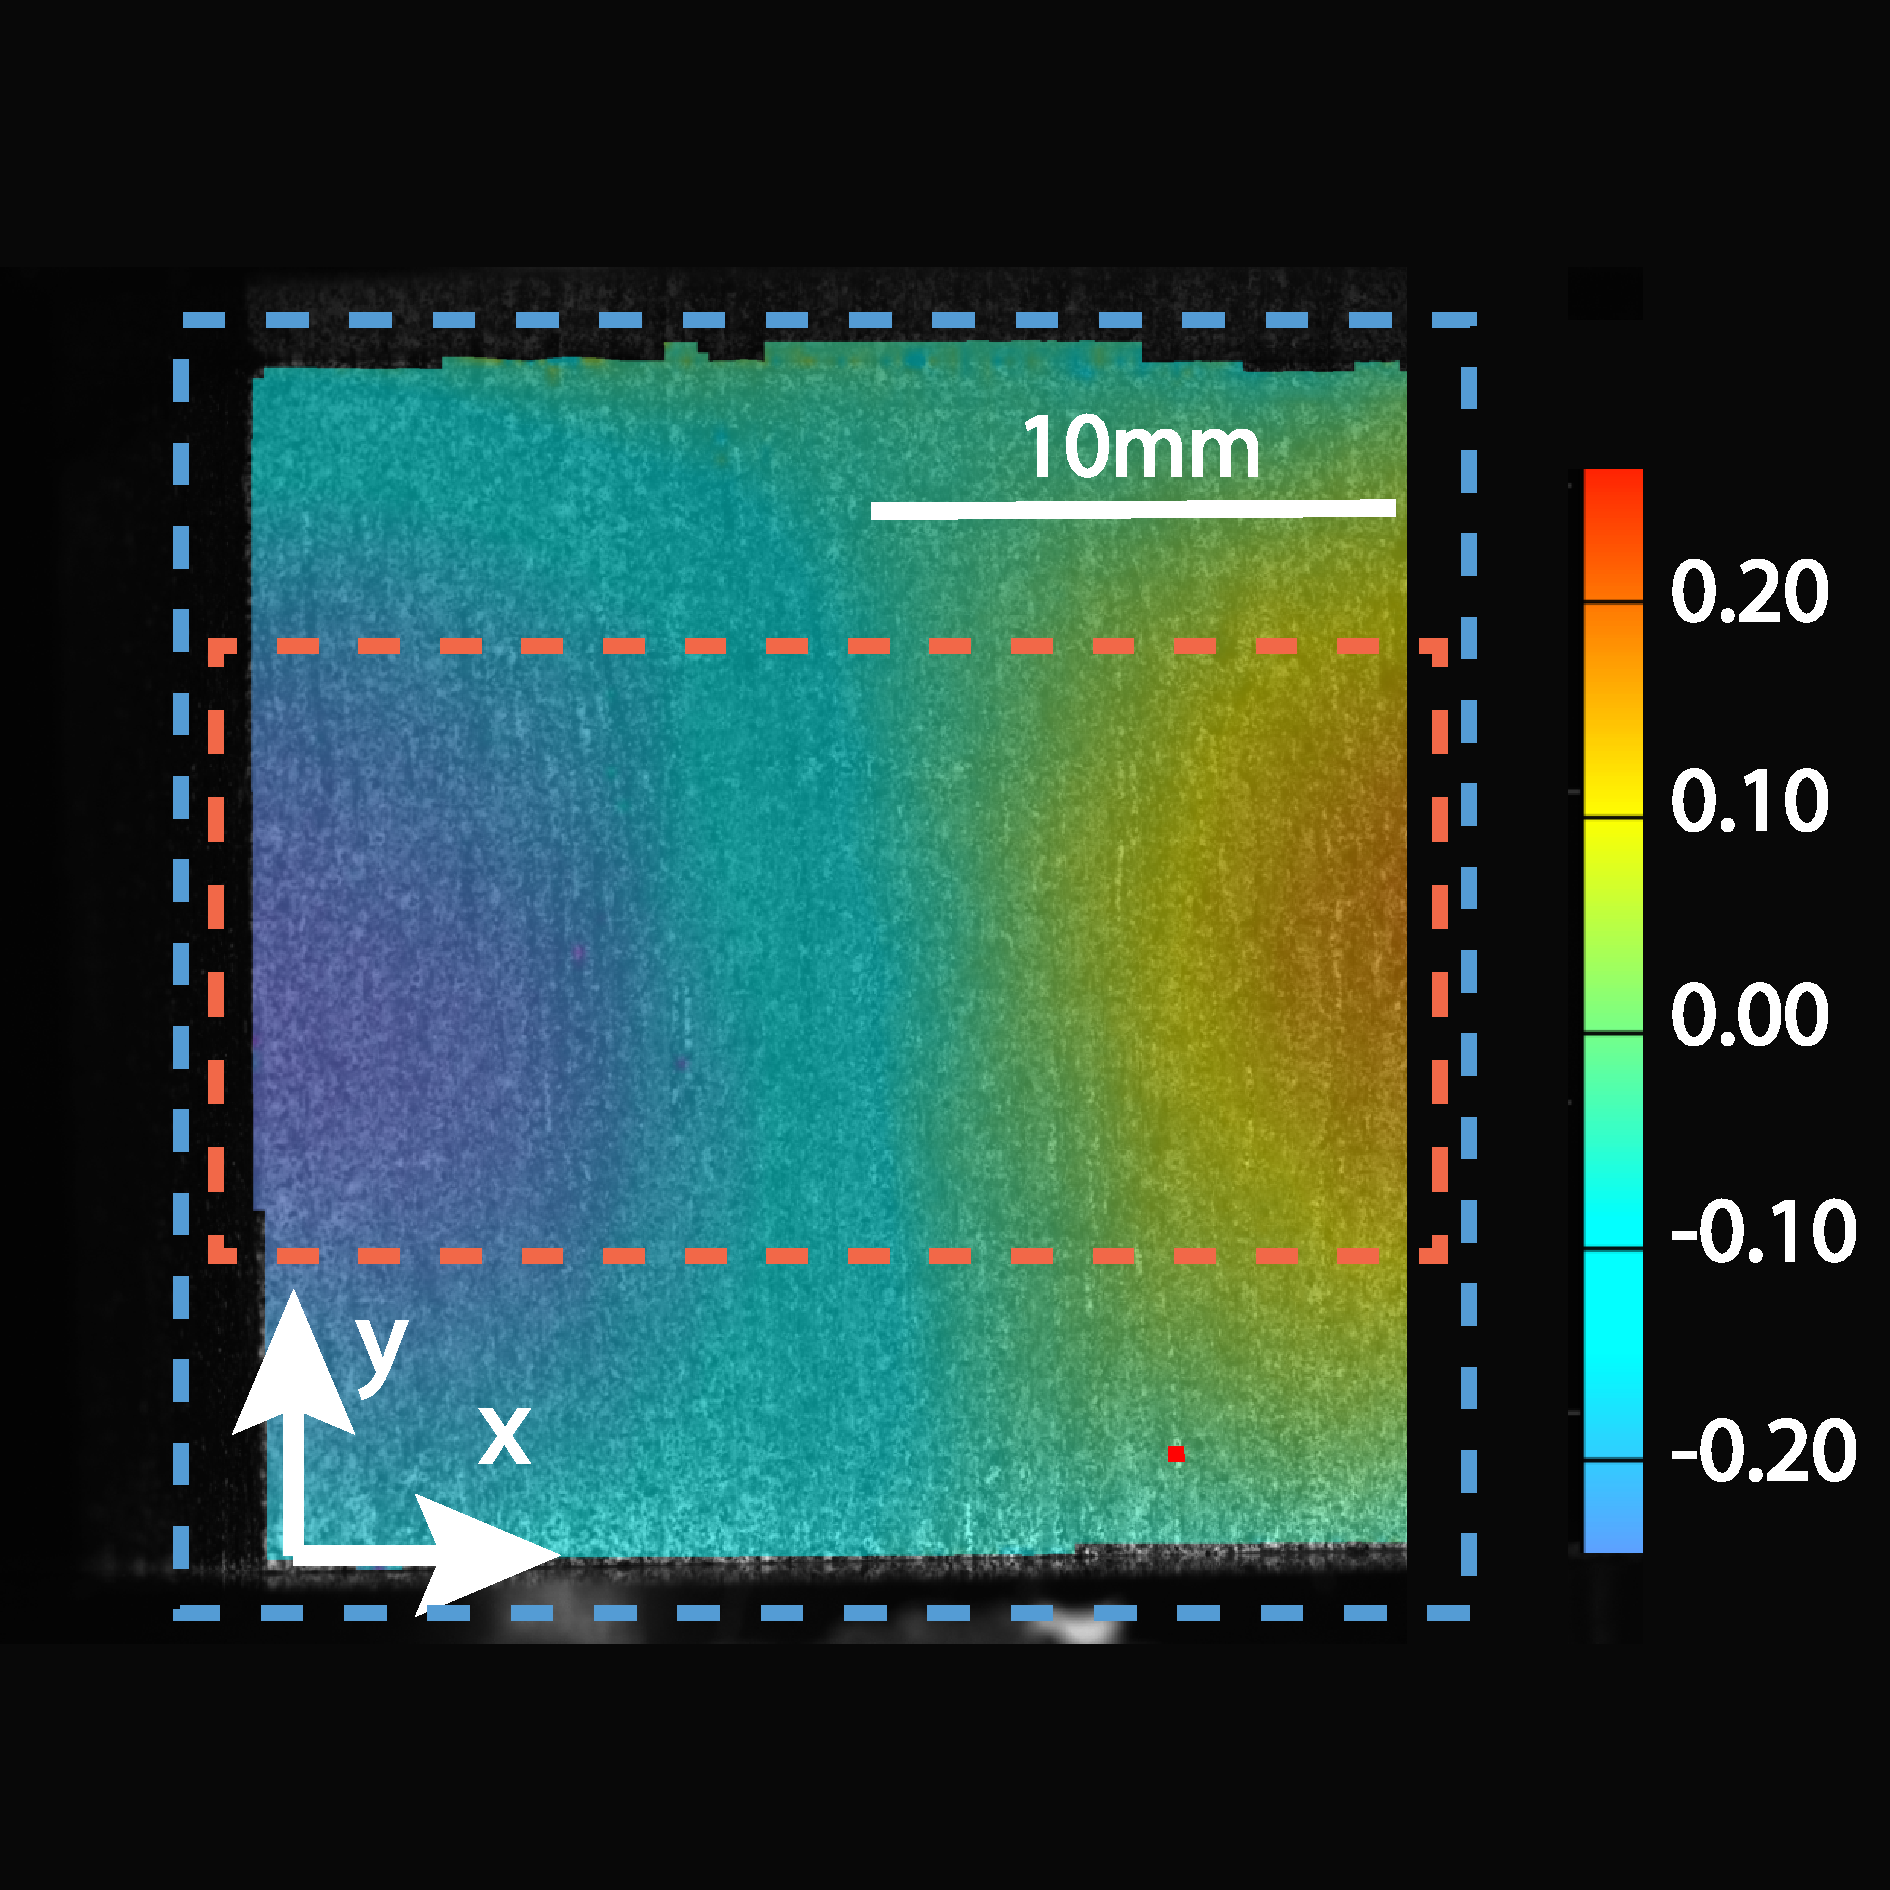
\includegraphics[width=\textwidth]{BarrellingPapper.pdf}
        \caption{}
        \label{fig:experiment}
    \end{subfigure}
    \hfill
    \hspace*{-20px}
    \begin{subfigure}[b]{0.4\textwidth}
        \centering
        \pgfplotsset{every axis legend/.append style={
		at={(0.5,1.03)},
		anchor=east}}
		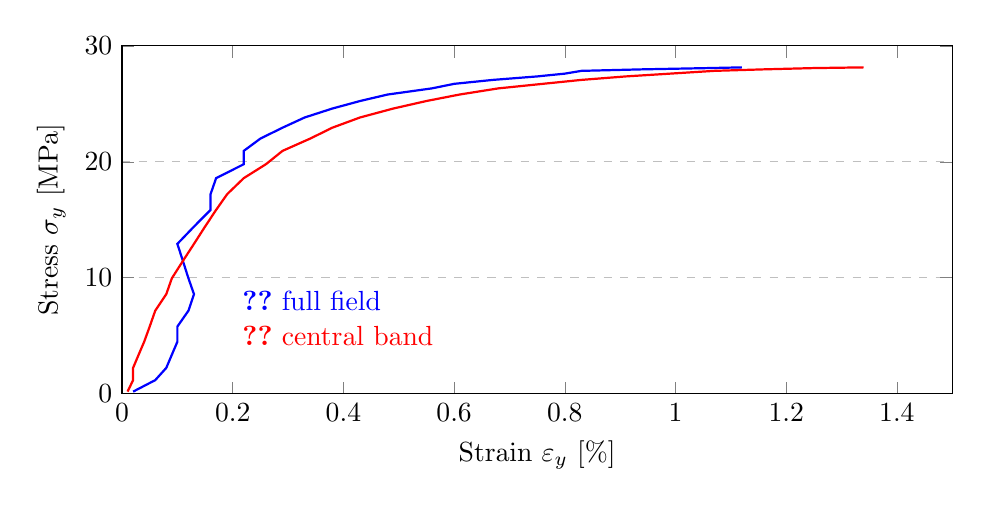
\begin{tikzpicture}
		\pgfplotstableread{
		stress	areaoi	totarea
		0.18	0.02	0.01
		1.17	0.06	0.02
		2.23	0.08	0.02
		3.36	0.09	0.03
		4.48	0.10	0.04
		5.79	0.10	0.05
		7.16	0.12	0.06
		8.59	0.13	0.08
		9.95	0.12	0.09
		11.45	0.11	0.11
		12.92	0.10	0.13
		14.41	0.13	0.15
		15.85	0.16	0.17
		17.21	0.16	0.19
		18.59	0.17	0.22
		19.79	0.22	0.26
		20.94	0.22	0.29
		22.00	0.25	0.34
		22.94	0.29	0.38
		23.82	0.33	0.43
		24.59	0.38	0.49
		25.24	0.43	0.55
		25.80	0.48	0.61
		26.33	0.56	0.68
		26.72	0.60	0.76
		27.06	0.67	0.83
		27.36	0.75	0.91
		27.60	0.80	0.99
		27.84	0.83	1.07
		27.97	0.94	1.16
		28.08	1.06	1.25
		28.14	1.12	1.34
		
		}\datatable
		
		
		
		
		\begin{axis}[no markers,
		name=plot0,height=6cm,width=\textwidth,
		    xlabel={Strain $\varepsilon_y$ [\%]},
		    ylabel={Stress $\sigma_y$ [MPa]},
		    xmin=0, xmax=1.5,
		    ymin=0, ymax=30,
		%     xtick={0,...,5},
		%    ytick={0,20,40,60,80},
		%     xticklabels={$0$,$0.2$,$0.4$,$0.6$,$0.8$, $1$}, 
		%     x tick label style={yshift=-1ex,
		%     rotate=45,anchor=east},
		    ymajorgrids=true,
		    grid style=dashed,
		]
		% \end{axis}    
		% \begin{axis}[legend pos=outer north east]
		 
		 
		    \addplot [thick, blue] table[x=areaoi,y=stress] {\datatable};
		    \label{ex1}
		%     \addlegendentry{Total surface area}
		    \addplot [thick, red] table[x=totarea,y=stress] {\datatable};
		    \label{ex2}
		%     \addlegendentry{Surface area of interest}
% 			\addplot [thin, red] coordinates {(0.0, 0.3) (0.28,28.0)};
% 			\addplot [thin, blue] coordinates {(0.05, 0.3) (0.25,28.0)};
\node at (axis cs:0.2,8) [anchor=west,blue] {\ref{ex1} full field};
\node at (axis cs:0.2,5) [anchor=west,red] {\ref{ex2} central band};
			
		
		\end{axis}
		
		\end{tikzpicture}		
        \caption{}
        \label{fig:explot}
    \end{subfigure}

\caption{(a) Vasa oak sample (b) Barrelling of an initially cubic shape.
(c) DSP image of Vasa oak sample during compressive testing including the
displacement field. (d) Experimental stress-strain curves for Vasa oak  sample
%, chosen surface area of interest(\ref{ex2}) and total surface area 
%(\ref{ex1})
.}
\label{fig:threegraphs}
\end{figure}













\subsection{Numerical model}





The finite element program COMSOL Multiphysics 4.4 \cite{Comsol} was used for
the numerical simulations.
A cube with unit dimensions was modelled with
3D solid elements.
The rig compliance was neglected since the platens were assumed to be rigid, leading to uniform normal displacement on the loaded surfaces.
The compressive loading was simulated as a downward vertical
displacement. The magnitude of this prescribed displacement was set to 0.01
which corresponds to an average compressive strain of  1\%.
A mesh refinement study showed that a $10\times10\times10$ mesh of quadratic
brick elements would provide sufficiently accurate results for the
purpose of this study.

\begin{figure}[h]
\centering
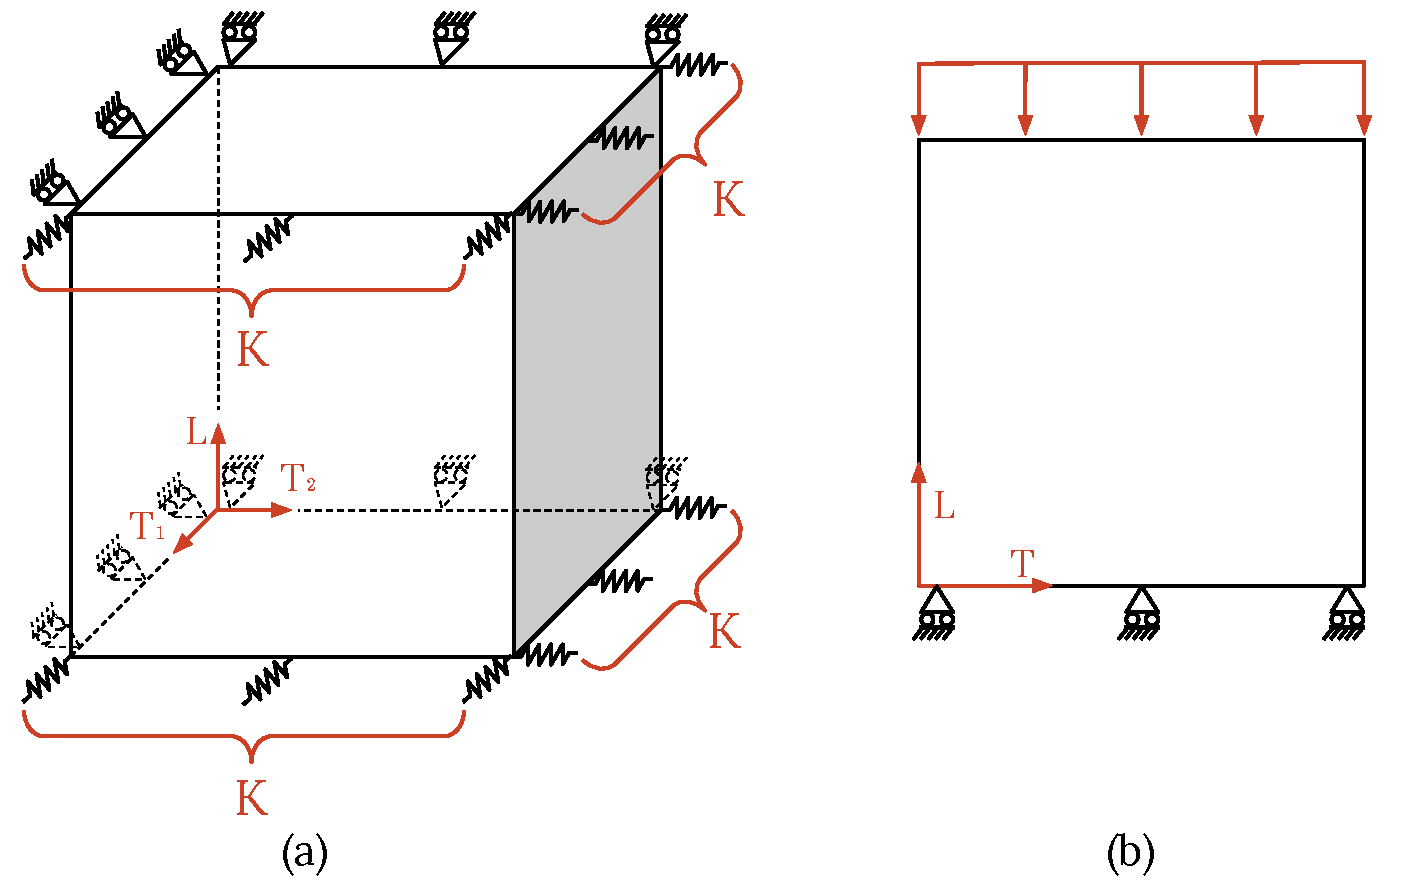
\includegraphics[width=8cm]{BarellingPaper.pdf}
\label{fig:Barrelling}
\caption{\label{fig:Barrelling} Model of cubic
sample used in the FEM simulation. 
(a) Horizontal boundary conditions and (b) vertical boundary conditions.}
\end{figure}

The main reason for the barrelling formation is the restraining friction between platens
and specimen \cite{Narayanasamy198821, kulkarni1969}. To simulate the effect of
friction, we have introduced line springs with spring constant $K$ (N/m$^2$) that represent the friction 
in the model. Those springs are evenly distributed along the edges on the top and the bottom of the cube as shown in Figure \ref{fig:Barrelling}.  
For $K=0$ (N/m$^2$) the displacement of the corresponding
edges is unconstrained, and for $K>0$ (N/m$^2$) the edges are partially
constrained up to the extreme case where the edges are completely constraint for
$K=\infty$ (N/m$^2$). It should be noted that the $K$ is not a physical friction
constant, such as the Coulomb friction over the contact area, but serves well to numerical simulate the effect of contact friction. 
In comparing the effects of barrelling on stiffness measurement, one would like
to use an easily measurable parameter, unlike the line spring constant or a
coefficient of static friction, $\mu$. An effect of friction closely related to
the barrel formation is the degree of slippage at the contact face. We define
this slippage as $\delta/\delta_{\mathrm{max}}$, where $\delta$ is the lateral
displacement and $\delta_{\mathrm{max}}$ is the maximum displacement,
corresponding to a maintained cuboid geometry.
Thus, $\delta/\delta_{\mathrm{max}}=0$ corresponds to no slippage with
$K=\infty$, and $\delta/\delta_{\mathrm{max}}=1$ corresponds to full slippage
with $K=0$ and $\mu=0$. The slippage $\delta$ is directly measurable from the
edge positions of the cube deformed cube, and $\delta_{\mathrm{max}}$ can be
calculated  from the deformed cuboid with no barrelling.


\subsection{Material input parameters}

Isotropic, transversely isotropic and orthotropic
linear elastic behaviour was investigated. Wood and composites materials are known to be anisotropic, although they are occasionally assumed to be transversely isotropic if two material axes have similar elastic properties compared the main material axis of fibre. The simplified isotropic case is added as reference. 
The relation between the elastic  properties are listed in
Table \ref{table:simulpar}. Two parameters $a$ and $b$ were introduced for a continuous transition between complete isotropy and transverse isotropy, while maintaining the symmetry conditions of the stiffness tensor. 
The first one , $a$, controls the relation between the stiffness in the
longitudinal and transverse directions as well as the corresponding Poisson's ratio.
The second one, $b$, controls the out-of-plane shear modulus.  
The remaining three Poisson's ratios were obtained from the symmetry
principle relations for the stiffness tensor \cite{hyer2009stress}. The parameters $a$ and $b$ were fitted to the  experimental elastic values of wooden and some composite materials in Table \ref{table:nonlin}. For the listed orthotropic wood and composite materials, $a=10$ and $b=2$ were found to provide a suitable compromise for a common transversely isotropic material. In the isotropic case, $a=1$ corresponding to uniform Young’s modulus $E$ and Poisson’s ratio $\nu$ in all directions. 
The orthotropic material was simulated using experimental input parameters
obtained from the experiments \cite{vorobyevcharacterisation}.


\subsection{Strain measuring methods}

Four realistic ways of measuring strain were considered in the simulations.
These strains are a result of the imposed displacement of the opposite faces of the unit cube of 0.01, corresponding to and average strain of 1\%.  The strains measured from the simulation results are:
\begin{itemize}
\item Average strain in the $x$ and $y$ directions over the entire analysed cube
face (Full field).
\item Average strains in the $x$ and $y$ directions over a centred area spanning
the width and covering 60\% of the total analysed cube face, as shown in Figure
\ref{fig:experiment}. This area of interest was chosen to represent DSP
measurements away from the constrained regions affected by restrained slippage
along the platens (Central band).
\item Average strain between two points in the $x$ and $y$ directions,
respectively, located close to the centre of the cube face. This corresponds to
the zone in which the strains are determined by the strain gauge as suggested in
the ASTM D143 standard (Strain gauges).
\cite{american2009standard}.
\item Average strain based directly on the 
measurements in the universal testing mashine from the
displacements of the compression platens (Basic method)
\end{itemize}


% Three strain measuring cases were taken intro account in simulation. The first
% case can be considered the same as taking the average dimensional changes of a
% sample. In particular the average strain from the total surface area was
% obtained and used as a value for obtaining axial stiffness $E_L$. In the
% second case, $50\%$ of cube surface (Figure \ref{fig:experiment}) was
% used to calculate the average strain corresponding to experimental measurement.
% Finally, in the third method the strain is measured between two points
% in horizontal and two points in vertical direction in the center of the sample
% as it is with the strain gauge based on ASTM-D143-94 standard
% \cite{american2009standard}.

\subsection{Experimental procedures}

Finally, the simulated results were compared with the results of an experiment
with \textit{Vasa} material.
An Instron universal testing machine with 100 kN load cell was used to carry out static tests. 
Special care was taken to prepare almost exactly cubic samples. The opposite faces of the cube were machined with a tolerance of 0.01 mm  of parallelity. 
The size of the samples was  $25\times25\times25$ mm\textsuperscript{3}.  
Initial tests were conducted on dummy wood specimens in order to find the approximate elastic loading range for all specimen orientations.
Full-field displacements were observed with a DSP equipment GOM Aramis stereo system 5M.
The distance to the measured object was 300 mm. The surfaces of specimens was spray-painted with speckles for better contrast. The applied force values were continuously recorded by the DSP system during testing, and stored together with the sampled images. The displacement rate was 0.5 mm per minute. 
Before measurement, the samples were conditioned at $23\,^{\circ}{\rm C}$ and 51\% relative humidity.
All the tests were performed without delay after the samples has been  removed from the conditioning chamber. The measurement recording frequency was 1 Hz. 
Each frame recorded by the DSP system was compared with the undeformed state in order to calculate the displacement and in-plane strain field. 
The total area of the region used in image analysis was a centered square
of 625 mm$\textsuperscript{2}$, covering one full face of the cubic sample.
The chosen region of interest is marked by the dashed line in Figure
\ref{fig:experiment}(b) and covers 50\% of the cube face. The acquired
strain fields were smoothed by averaging of each data pixel with $3\times3$ surrounding pixels in order to avoid 
undesired spike artifacts in the measured strain field.
The strain determined by DSP in the loading direction was plotted against the
applied stress, as exemplified in Figure \ref{fig:explot}(c). The choice of strain measure
is the subject of a later discussion.
The Poisson's ratios $\nu_{xy}$ for all corresponding orthotropic planes were
calculated as the negative ratio between the average transverse
$\varepsilon_{x}$ (passive ) and normal $\varepsilon_{y}$ (compressive and
active) strains.


\begin{center}% note that \centering uses less vspace...
\begin{figure}[!ht]
\pgfplotsset{every axis legend/.append style={
		at={(0.5,1.03)},
		anchor=north}}

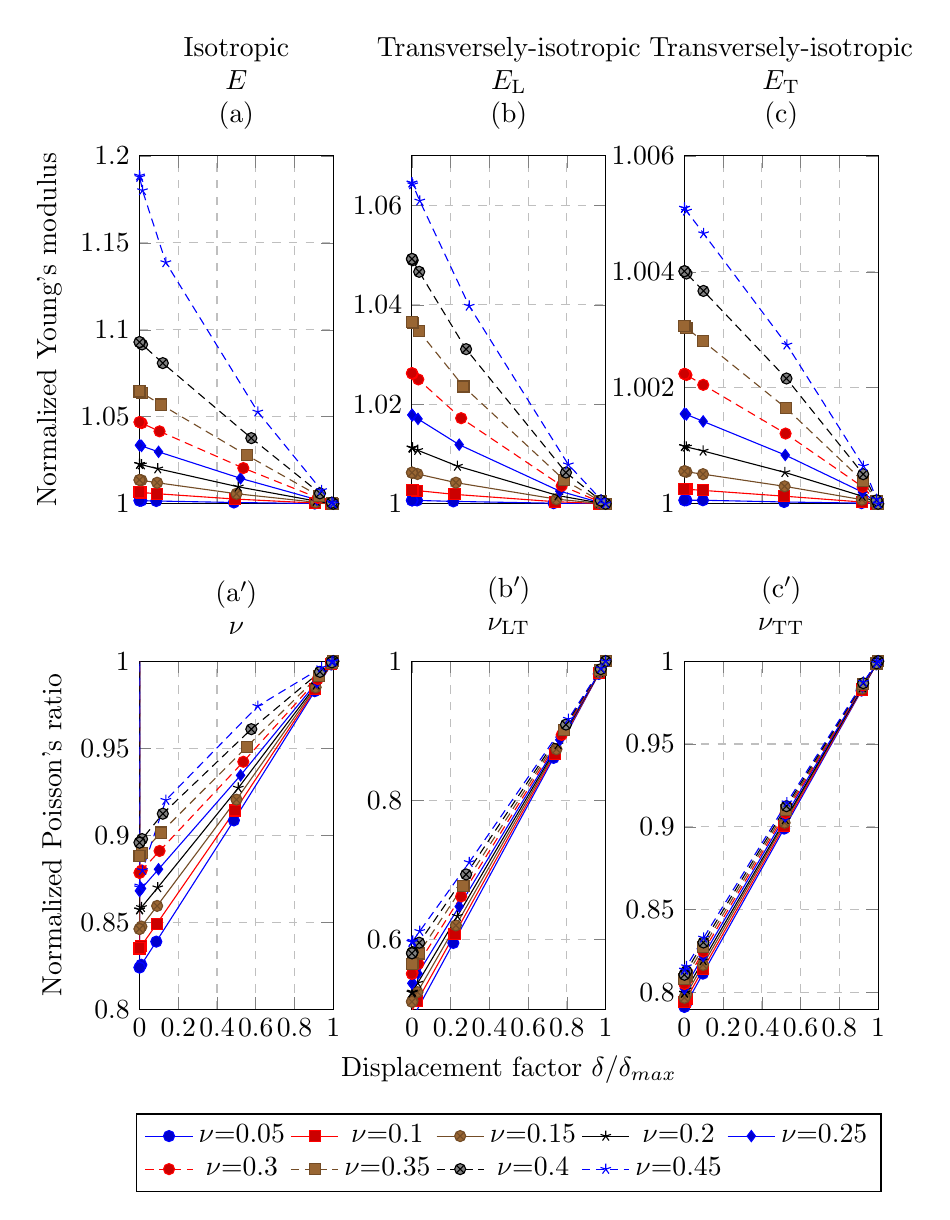
\begin{tikzpicture}[scale=1]

	\pgfplotstableread{
K	s1	0.05	s2	0.1	s3	0.15	s4	0.2	s5	0.25	s6	0.3	s7	0.35	s8	0.4	s9	0.45
1	1	1	1	1	1	1	1	1	1	1	1	1	1	1	1	1	1	1
2	1.00001	0.98959	1.00004	0.98983	1.00009	0.99013	1.00016	0.99049	1.00025	0.99091	1.00036	0.99141	1.00049	0.99201	1.00064	0.99273	1.00081	0.99366
3	1.0001	0.90485	1.00039	0.90684	1.00086	0.90934	1.00151	0.91237	1.00234	0.916	1.00335	0.92031	1.00455	0.92545	1.00598	0.93174	1.00768	0.94003
4	1.00071	0.48743	1.00269	0.49329	1.00574	0.50078	1.00972	0.51016	1.0146	0.52174	1.02051	0.53607	1.02786	0.55404	1.03771	0.57742	1.05282	0.61085
5	1.00157	0.08684	1.00577	0.08872	1.01207	0.09119	1.02012	0.09437	1.02983	0.09844	1.04161	0.1037	1.05701	0.11069	1.08084	0.12049	1.13869	0.1361
6	1.00176	0.00942	1.00647	0.00964	1.01348	0.00994	1.02243	0.01031	1.03322	0.0108	1.04635	0.01144	1.0637	0.0123	1.09157	0.01353	1.18008	0.01554
7	1.00178	0.00095009	1.00654	0.00097274	1.01364	0.001	1.02269	0.00104	1.0336	0.00109	1.04688	0.00116	1.06446	0.00124	1.09282	0.00137	1.18771	0.00158
8	1.00179	9.50903E-05	1.00655	9.73593E-05	1.01366	0.000100348	1.02272	0.000104217	1.03364	0.000109217	1.04693	0.000115754	1.06454	0.00012456	1.09295	0.000137156	1.18856	0.000157846

}\datatable

\pgfplotstableread{
K	s1	0.05	s2	0.1	s3	0.15	s4	0.2	s5	0.25	s6	0.3	s7	0.35	s8	0.4	s9	0.45
0	1	1	1	1	1	1	1	1	1	1	1	1	1	1	1	1	1	1
0.001	1.00001	0.96454	1.00004	0.96576	1.00009	0.96707	1.00016	0.96846	1.00025	0.96993	1.00036	0.97149	1.00049	0.97314	1.00064	0.97488	1.00081	0.97672
0.01	1.0001	0.73119	1.00041	0.73827	1.00092	0.74597	1.00163	0.75431	1.00252	0.76334	1.0036	0.77311	1.00485	0.78368	1.00627	0.79513	1.00786	0.80754
0.1	1.00047	0.21384	1.00188	0.22002	1.00424	0.227	1.00757	0.23491	1.01188	0.2439	1.01721	0.25418	1.02359	0.26598	1.0311	0.27966	1.03978	0.29565
1	1.00066	0.02648	1.00264	0.02744	1.00598	0.02853	1.01076	0.02979	1.01706	0.03126	1.02501	0.03296	1.03479	0.03498	1.04666	0.03739	1.06095	0.04031
10	1.00068	0.00271	1.00274	0.00281	1.00623	0.00293	1.01121	0.00306	1.0178	0.00322	1.02614	0.0034	1.03644	0.00361	1.04899	0.00387	1.06421	0.00418
100	1.00068	0.000271937	1.00275	0.000282014	1.00625	0.0002936	1.01126	0.000306985	1.01787	0.000322546	1.02625	0.000340787	1.03661	0.000362391	1.04924	0.000388305	1.06455	0.000419892
1000	1.00068	2.72003E-05	1.00275	2.82085E-05	1.00625	2.93678E-05	1.01126	3.07069E-05	1.01788	0.000032264	1.02627	3.40892E-05	1.03663	3.62509E-05	1.04926	3.88442E-05	1.06458	4.20052E-05


}\datatableA

\pgfplotstableread{
K	s1	0.05	s2	0.1	s3	0.15	s4	0.2	s5	0.25	s6	0.3	s7	0.35	s8	0.4	s9	0.45
0	1	1	1	1	1	1	1	1	1	1	1	1	1	1	1	1	1	1
0.001	1	0.99079	1	0.99096	1.00001	0.99114	1.00002	0.99132	1.00002	0.99151	1.00004	0.9917	1.00005	0.9919	1.00006	0.9921	1.00008	0.9923
0.01	1.00001	0.91454	1.00003	0.91559	1.00007	0.91669	1.00013	0.91784	1.0002	0.91904	1.00029	0.92028	1.00039	0.92157	1.00051	0.92291	1.00065	0.9243
0.1	1.00003	0.51477	1.00013	0.51597	1.0003	0.51733	1.00054	0.51887	1.00084	0.52059	1.00121	0.52248	1.00165	0.52456	1.00216	0.52682	1.00274	0.52927
1	1.00006	0.0957	1.00023	0.09591	1.00051	0.09618	1.00091	0.09651	1.00142	0.0969	1.00205	0.09735	1.0028	0.09787	1.00367	0.09846	1.00466	0.09912
10	1.00006	0.01047	1.00025	0.01049	1.00055	0.01052	1.00098	0.01056	1.00154	0.0106	1.00222	0.01065	1.00303	0.01071	1.00397	0.01078	1.00505	0.01086
100	1.00006	0.00106	1.00025	0.00106	1.00056	0.00106	1.00099	0.00107	1.00155	0.00107	1.00224	0.00108	1.00306	0.00108	1.00401	0.00109	1.0051	0.0011
1000	1.00006	0.000105788	1.00025	0.000106007	1.00056	0.000106301	1.00099	0.00010667	1.00155	0.000107116	1.00224	0.000107641	1.00306	0.000108246	1.00401	0.000108934	1.0051	0.000109708



}\datatableB

\pgfplotstableread{
K	p1	0.05	p2	0.1	p3	0.15	p4	0.2	p5	0.25	p6	0.3	p7	0.35	p8	0.4	p9	0.45
1	1	1	1	1	1	1	1	1	1	1	1	1	1	1	1	1	1	1
2	0.99811	0.98959	0.99822	0.98983	0.99836	0.99013	0.99851	0.99049	0.99869	0.99091	0.99889	0.99141	0.99911	0.99201	0.99935	0.99273	0.99962	0.99366
3	0.98278	0.90485	0.98381	0.90684	0.98503	0.90934	0.98641	0.91237	0.98798	0.916	0.98973	0.92031	0.99168	0.92545	0.99387	0.93174	0.99633	0.94003
4	0.90847	0.48743	0.91417	0.49329	0.92042	0.50078	0.92716	0.51016	0.93439	0.52174	0.94218	0.53607	0.95081	0.55404	0.96094	0.57742	0.97419	0.61085
5	0.8388	0.08684	0.84892	0.08872	0.85932	0.09119	0.86987	0.09437	0.88042	0.09844	0.89092	0.1037	0.90149	0.11069	0.91232	0.12049	0.92012	0.1361
6	0.82548	0.00942	0.8364	0.00964	0.84747	0.00994	0.85851	0.01031	0.86932	0.0108	0.87971	0.01144	0.88953	0.0123	0.89776	0.01353	0.87979	0.01554
7	0.82403	0.00095009	0.83503	0.00097274	0.84617	0.001	0.85725	0.00104	0.86807	0.00109	0.87843	0.00116	0.8881	0.00124	0.89587	0.00137	0.87093	0.00158
8	0.82388	9.50903E-05	0.83489	9.73593E-05	0.84603	0.000100348	0.85713	0.000104217	0.86795	0.000109217	0.8783	0.000115754	0.88795	0.00012456	0.89568	0.000137156	0.86991	0.000157846
9	1.00179	9.50903E-05	1.00655	9.73593E-05	1.01366	0.000100348	1.02272	0.000104217	1.03364	0.000109217	1.04693	0.000115754	1.06454	0.00012456	1.09295	0.000137156	1.18856	0.000157846


}\datatableC

\pgfplotstableread{
K	p1	0.05	p2	0.1	p3	0.15	p4	0.2	p5	0.25	p6	0.3	p7	0.35	p8	0.4	p9	0.45
0	1	1	1	1	1	1	1	1	1	1	1	1	1	1	1	1	1	1
0.001	0.98163	0.96454	0.98255	0.96576	0.9835	0.96707	0.98446	0.96846	0.98546	0.96993	0.98647	0.97149	0.98752	0.97314	0.98859	0.97488	0.98969	0.97672
0.01	0.86103	0.73119	0.86719	0.73827	0.87356	0.74597	0.88015	0.75431	0.88696	0.76334	0.89402	0.77311	0.90133	0.78368	0.90892	0.79513	0.9168	0.80754
0.1	0.59508	0.21384	0.60748	0.22002	0.62028	0.227	0.63358	0.23491	0.64744	0.2439	0.66198	0.25418	0.67731	0.26598	0.69357	0.27966	0.7109	0.29565
1	0.49897	0.02648	0.51154	0.02744	0.52436	0.02853	0.5375	0.02979	0.55107	0.03126	0.56517	0.03296	0.57992	0.03498	0.59544	0.03739	0.61191	0.04031
10	0.48675	0.00271	0.49923	0.00281	0.51193	0.00293	0.52492	0.00306	0.53829	0.00322	0.55215	0.0034	0.5666	0.00361	0.58178	0.00387	0.59782	0.00418
100	0.48549	2.72E-04	0.49796	2.82E-04	0.51065	2.94E-04	0.52362	3.07E-04	0.53697	3.23E-04	0.55081	3.41E-04	0.56523	3.62E-04	0.58036	3.88E-04	0.59635	4.20E-04
1000	0.48536	2.72E-05	0.49784	2.82E-05	0.51052	2.94E-05	0.52349	3.07E-05	0.53684	3.23E-05	0.55067	3.41E-05	0.56509	3.63E-05	0.58022	3.88E-05	0.5962	4.20E-05



}\datatableD

\pgfplotstableread{
K	p1	0.05	p2	0.1	p3	0.15	p4	0.2	p5	0.25	p6	0.3	p7	0.35	p8	0.4	p9	0.45
0	1	1	1	1	1	1	1	1	1	1	1	1	1	1	1	1	1	1
0.001	0.9981	0.99079	0.99818	0.99096	0.99826	0.99114	0.99835	0.99151	0.99844	0.99151	0.99853	0.9917	0.99862	0.9919	0.99871	0.9921	0.9988	0.9923
0.01	0.98229	0.91454	0.98288	0.91559	0.98348	0.91669	0.98409	0.91904	0.98473	0.91904	0.98539	0.92028	0.98606	0.92157	0.98675	0.92291	0.98746	0.9243
0.1	0.89895	0.51477	0.90071	0.51597	0.90253	0.51733	0.90441	0.52059	0.90634	0.52059	0.90833	0.52248	0.91038	0.52456	0.9125	0.52682	0.91467	0.52927
1	0.81141	0.0957	0.81404	0.09591	0.81668	0.09618	0.81934	0.0969	0.82202	0.0969	0.82472	0.09735	0.82745	0.09787	0.83021	0.09846	0.833	0.09912
10	0.79351	0.01047	0.79628	0.01049	0.79903	0.01052	0.80179	0.0106	0.80455	0.0106	0.80732	0.01065	0.81011	0.01071	0.8129	0.01078	0.81571	0.01086
100	0.79153	0.00106	0.7943	0.00106	0.79707	0.00106	0.79984	0.00107	0.8026	0.00107	0.80538	0.00108	0.80816	0.00108	0.81095	0.00109	0.81376	0.0011
1000	0.79133	0.000105788	0.7941	0.000106007	0.79687	0.000106301	0.79964	0.000107116	0.8024	0.000107116	0.80518	0.000107641	0.80796	0.000108246	0.81075	0.000108934	0.81356	0.000109708


}\datatableE



\begin{axis}[
name=plot0,height=6cm,width=\textwidth/3,
	align =center,
    title={Isotropic\\$E$\\(a)},
%    xlabel={Temperature [\textcelsius]},
    ylabel={Normalized Young's modulus},
    xmin=0, xmax=1,
    ymin=1, ymax=1.2,
%     xtick={1,...,9},
%    ytick={0,20,40,60,80},
    xticklabels={},
    ymajorgrids=true,
    xmajorgrids=true,
    grid style=dashed,
]
% \end{axis}
% \begin{axis}[legend pos=outer north east]


    \addplot table[y=s1,x=0.05] {\datatable};
%     \addlegendentry{$\nu$=0.05}
    \addplot table[y=s2,x=0.1] {\datatable};
%     \addlegendentry{$\nu$=0.1}
    \addplot table[y=s3,x=0.15] {\datatable};
%     \addlegendentry{$\nu$=0.15}
    \addplot table[y=s4,x=0.2] {\datatable};
%     \addlegendentry{$\nu$=0.2}
    \addplot table[y=s5,x=0.25] {\datatable};
%     \addlegendentry{$\nu$=0.25}
    \addplot table[y=s6,x=0.3] {\datatable};
%     \addlegendentry{$\nu$=0.3}
    \addplot table[y=s7,x=0.35] {\datatable};
%     \addlegendentry{$\nu$=0.35}
    \addplot table[y=s8,x=0.4] {\datatable};
%     \addlegendentry{$\nu$=0.4}
    \addplot table[y=s9,x=0.45] {\datatable};
%     \addlegendentry{$\nu$=0.45}

% \draw	(70,160) node{{Isotropic}};
\end{axis}

\begin{axis}[
name=plot1,at={($(plot0.east)+(1cm,0)$)},anchor=west,
height=6cm,width=\textwidth/3,
align =center,
title={Transversely-isotropic\\$E_{\mathrm{L}}$\\(b)},
%    xlabel={Temperature [\textcelsius]},
%    ylabel={Measured stiffness [Pa]},
    xmin=0, xmax=1,
    ymin=1, ymax=1.07,
    yticklabel style={/pgf/number format/fixed,
                  /pgf/number format/precision=3},
%     xtick={1,...,9},
%    ytick={0,20,40,60,80},
%     xticklabels={$0$,$0.001$,$0.01$,$0.1$,$1$, $10$, $100$,
%     $1000$, $\infty$},
    xticklabels={},
    ymajorgrids=true,
    xmajorgrids=true,
    grid style=dashed,
]

    \addplot table[y=s1,x=0.05] {\datatableA};
%     \addlegendentry{$\nu$=0.05}
    \addplot table[y=s2,x=0.1] {\datatableA};
%     \addlegendentry{$\nu$=0.1}
    \addplot table[y=s3,x=0.15] {\datatableA};
%     \addlegendentry{$\nu$=0.15}
    \addplot table[y=s4,x=0.2] {\datatableA};
%     \addlegendentry{$\nu$=0.2}
    \addplot table[y=s5,x=0.25] {\datatableA};
%     \addlegendentry{$\nu$=0.25}
    \addplot table[y=s6,x=0.3] {\datatableA};
%     \addlegendentry{$\nu$=0.3}
    \addplot table[y=s7,x=0.35] {\datatableA};
%     \addlegendentry{$\nu$=0.35}
    \addplot table[y=s8,x=0.4] {\datatableA};
%     \addlegendentry{$\nu$=0.4}
    \addplot table[y=s9,x=0.45] {\datatableA};
%     \addlegendentry{$\nu$=0.45}


\end{axis}

\begin{axis}[
	name=plot2,at={($(plot1.east)+(1cm,0)$)},anchor=west, height=6cm,width=\textwidth/3,
align =center,
title={Transversely-isotropic\\$E_{\mathrm{T}}$\\(c)},
%    xlabel={Temperature [\textcelsius]},
%    ylabel={Measured stiffness [Pa]},
    xmin=0, xmax=1,
    ymin=1, ymax=1.006,
    yticklabel style={/pgf/number format/fixed,
                  /pgf/number format/precision=3},
%     xtick={1,...,9},
%    ytick={0,20,40,60,80},
    xticklabels={},
    ymajorgrids=true,
    xmajorgrids=true,
    grid style=dashed,
    bar shift=0pt
]

    \addplot table[y=s1,x=0.05] {\datatableB};
%     \addlegendentry{$\nu$=0.05}
    \addplot table[y=s2,x=0.1] {\datatableB};
%     \addlegendentry{$\nu$=0.1}
    \addplot table[y=s3,x=0.15] {\datatableB};
%     \addlegendentry{$\nu$=0.15}
    \addplot table[y=s4,x=0.2] {\datatableB};
%     \addlegendentry{$\nu$=0.2}
    \addplot table[y=s5,x=0.25] {\datatableB};
%     \addlegendentry{$\nu$=0.25}
    \addplot table[y=s6,x=0.3] {\datatableB};
%     \addlegendentry{$\nu$=0.3}
    \addplot table[y=s7,x=0.35] {\datatableB};
%     \addlegendentry{$\nu$=0.35}
    \addplot table[y=s8,x=0.4] {\datatableB};
%     \addlegendentry{$\nu$=0.4}
    \addplot table[y=s9,x=0.45] {\datatableB};
%     \addlegendentry{$\nu$=0.45}


\end{axis}

\begin{axis}[name=plot3,at={($(plot0.south)-(0,2cm)$)},anchor=north,
height=6cm,width=\textwidth/3,
align =center,
title={(a\textprime)\\ $\nu$},
%    xlabel={Temperature [\textcelsius]},
    ylabel={Normalized Poisson's ratio},
    xmin=0, xmax=1,
    ymin=0.8, ymax=1,
%     xtick={1,...,9},
%    ytick={0,20,40,60,80},
%     xticklabels={$0$,$0.001$,$0.01$,$0.1$,$1$, $10$, $100$,
%     $1000$, $\infty$},
%     x tick label style={yshift=-1ex,
%     rotate=45,anchor=east},
    ymajorgrids=true,
    xmajorgrids=true,
    grid style=dashed,
]
% \end{axis}
% \begin{axis}[legend pos=outer north east]


    \addplot table[y=p1,x=0.05] {\datatableC};
%     \addlegendentry{$\nu$=0.05}
    \addplot table[y=p2,x=0.1] {\datatableC};
%     \addlegendentry{$\nu$=0.1}
    \addplot table[y=p3,x=0.15] {\datatableC};
%     \addlegendentry{$\nu$=0.15}
    \addplot table[y=p4,x=0.2] {\datatableC};
%     \addlegendentry{$\nu$=0.2}
    \addplot table[y=p5,x=0.25] {\datatableC};
%     \addlegendentry{$\nu$=0.25}
    \addplot table[y=p6,x=0.3] {\datatableC};
%     \addlegendentry{$\nu$=0.3}
    \addplot table[y=p7,x=0.35] {\datatableC};
%     \addlegendentry{$\nu$=0.35}
    \addplot table[y=p8,x=0.4] {\datatableC};
%     \addlegendentry{$\nu$=0.4}
    \addplot table[y=p9,x=0.45] {\datatableC};
%     \addlegendentry{$\nu$=0.45}
\end{axis}

\begin{axis}[legend style={at={(0.5,-0.3)}, legend columns=5, anchor=north},
	name=plot4,at={($(plot1.south)-(0,2cm)$)},anchor=north,
	height=6cm,width=\textwidth/3, align=center,
title={(b\textprime) \\ $\nu_{\mathrm{LT}}$},
    xlabel={Displacement factor $\delta/\delta_{max}$},
%    ylabel={Measured stiffness [Pa]},
    xmin=0, xmax=1,
    ymin=0.5, ymax=1,
    yticklabel style={/pgf/number format/fixed,
                  /pgf/number format/precision=3},
%     xtick={1,...,9},
%    ytick={0,20,40,60,80},
%     xticklabels={$0$,$0.001$,$0.01$,$0.1$,$1$, $10$, $100$,
%     $1000$, $\infty$},
%     x tick label style={yshift=-1ex,
%         rotate=45,anchor=east},
    ymajorgrids=true,
    xmajorgrids=true,
    grid style=dashed,
    bar shift=0pt
]

    \addplot table[y=p1,x=0.05] {\datatableD};
     \addlegendentry{$\nu$=0.05}
    \addplot table[y=p2,x=0.1] {\datatableD};
     \addlegendentry{$\nu$=0.1}
    \addplot table[y=p3,x=0.15] {\datatableD};
     \addlegendentry{$\nu$=0.15}
    \addplot table[y=p4,x=0.2] {\datatableD};
     \addlegendentry{$\nu$=0.2}
    \addplot table[y=p5,x=0.25] {\datatableD};
     \addlegendentry{$\nu$=0.25}
    \addplot table[y=p6,x=0.3] {\datatableD};
     \addlegendentry{$\nu$=0.3}
    \addplot table[y=p7,x=0.35] {\datatableD};
     \addlegendentry{$\nu$=0.35}
    \addplot table[y=p8,x=0.4] {\datatableD};
     \addlegendentry{$\nu$=0.4}
    \addplot table[y=p9,x=0.45] {\datatableD};
     \addlegendentry{$\nu$=0.45}

\end{axis}


\begin{axis}[
	name=plot5,at={($(plot2.south)-(0,2cm)$)},anchor=north,
	height=6cm,width=\textwidth/3, align=center,
	 title={(c\textprime)\\ $\nu_{\mathrm{TT}}$},
%    xlabel={Temperature [\textcelsius]},
%    ylabel={Measured stiffness [Pa]},
    xmin=0, xmax=1,
    ymin=0.79, ymax=1.,
    yticklabel style={/pgf/number format/fixed,
                  /pgf/number format/precision=3},
%     xtick={1,...,9},
%    ytick={0,20,40,60,80},
%     xticklabels={$0$,$0.001$,$0.01$,$0.1$,$1$, $10$, $100$,
%     $1000$, $\infty$},
%         x tick label style={yshift=-1ex,
%         rotate=45,anchor=east		},
    ymajorgrids=true,
    xmajorgrids=true,
    grid style=dashed,
    bar shift=0pt
]

    \addplot table[y=p1,x=0.05] {\datatableE};
%     \addlegendentry{$\nu$=0.05}
    \addplot table[y=p2,x=0.1] {\datatableE};
%     \addlegendentry{$\nu$=0.1}
    \addplot table[y=p3,x=0.15] {\datatableE};
%     \addlegendentry{$\nu$=0.15}
    \addplot table[y=p4,x=0.2] {\datatableE};
%     \addlegendentry{$\nu$=0.2}
    \addplot table[y=p5,x=0.25] {\datatableE};
%     \addlegendentry{$\nu$=0.25}
    \addplot table[y=p6,x=0.3] {\datatableE};
%     \addlegendentry{$\nu$=0.3}
    \addplot table[y=p7,x=0.35] {\datatableE};
%     \addlegendentry{$\nu$=0.35}
    \addplot table[y=p8,x=0.4] {\datatableE};
%     \addlegendentry{$\nu$=0.4}
    \addplot table[y=p9,x=0.45] {\datatableE};
%     \addlegendentry{$\nu$=0.45}

\end{axis}


\end{tikzpicture}


\captionsetup{justification=centering}
\caption{Simulated and normalized Young's moduli and Poisson's ratio of
isotropic material ($a=1$) and transversely isotropic
material ($a=10$; $b=2$) with initial Poisson's ratio ($\nu$) versus
displacement factor.}

\label{fig:isovstriso}
\end{figure}

\end{center}


\color{black}


\section{Results and discussion}
The simulated strain results can be used to compare the errors in the estimated elastic parameters and the suitability of the different strain measures.
There is an unlimited number of parametric simulations that could be done, and we limit ourselves to a set that we consider relevant for wood and composite applications. 



\subsection{ Barrelling in Isotropic and Transversely isotropic material}


Elastic moduli and Poisson’s ratios normalized with the correct values are presented in Figure \ref{fig:isovstriso} as a function of relative slippage due to platen friction and Poisson’s ratios for the isotropic case (a) and the transversely isotropic case, (b) and (c). 
For all simulations the
barrelling is leading to an overestimation of the Young's moduli, as shown in Figures \ref{fig:isovstriso}(a), (b) and (c). This is caused by the perturbed strain field in the area close to the upper and lower edges, where constrained material has a stiffer response. Noting the difference in scales of the $y$-axes, it is clear that the errors in Young’s modulus is significantly higher for the isotropic case than for the transversely isotropic case. This effect is larger for LT plane (loading in the L direction) than for the TT plane, comparing Figures \ref{fig:isovstriso}(b) and (c). As expected, the error is becomes larger for increasing Poisson’s ratio $\nu$. The perturbed zones are shown in Figure \ref{fig:Error} in term of local error on the examined face, where the modulus is determined simply as $\sigma_y/{\epsilon_y(x,y)}$ in (a), (b) and (c), and the Poisson ratio is determined as $-\epsilon_x/{\epsilon_y(x,y)}$. 
In general, for increasing Poisson's ratio, the error becomes larger. 
For the transversely isotropic material in Figures
\ref{fig:isovstriso} (b) and (c) the error in Young's moduli is less in
transverse direction T than in the axial direction L.
This difference in behavior can be discussed by examining the spatial variation of elastic parameters determined from strain fields for isotropic and 
transversely isotropic materials shown in Figure 
\ref{fig:Error} (a-c). One can
observe the patterns of the constraining effect that originate from the top
and bottom of the cube face where the sample is in contact with the platens. The constraining effect is significant in the zones within $20\%$ of height
from the horizontal edges of the model. 
Figure \ref{fig:isovstriso} (a’) shows that the relative error for the
Poisson's ratio is smaller in isotropic material than in transversely isotropic
materials in Figure \ref{fig:isovstriso} (b’,c’). This can also be observed
by the with the corresponding strain ratio field in Figure \ref{fig:Error} (a\textprime).

\begin{figure}[h]
\centering
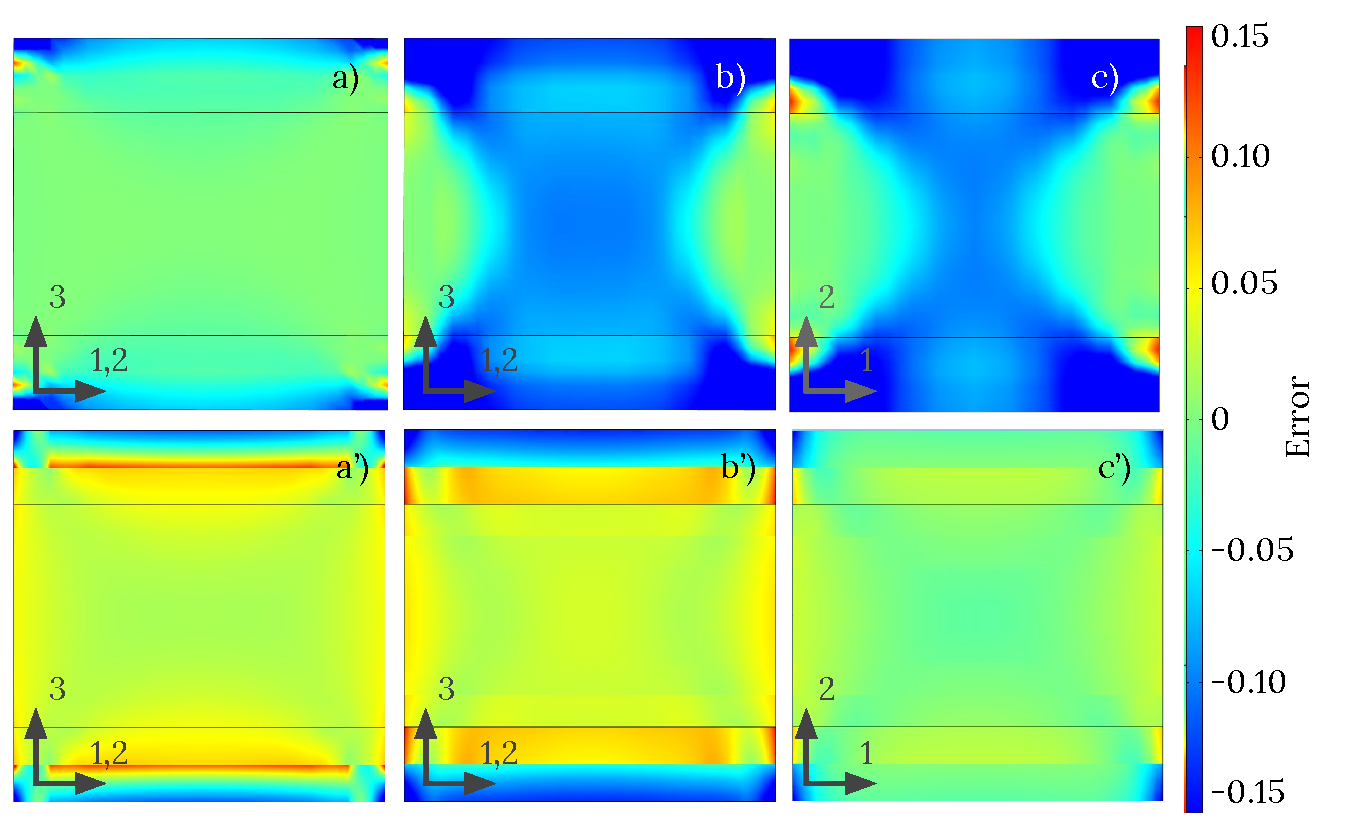
\includegraphics[width=\textwidth]{BarellingError.pdf}
\label{fig:Error}
\caption{\label{fig:Error} Simulated results of error for measured Young's
moduli and Poisson's ratio of isotropic and transversely isotropic
material. ($K=0.1; \nu=0.3; \delta/\delta_{max}\approx0.2$)}

\end{figure}

The green zones corresponding to vanishing error is found in the central band of
the numerical model. For the transversely isotropic cases, Figures
\ref{fig:isovstriso} (b\textprime), (LT plane) and (c\textprime), (TT plane) the error is
non-negligible also in the central part of the cube face. The effect is stronger for the LT plane, where the perturbed zones extends over a larger area.
For instance, for the displacement factor $\delta/\delta_{max}\approx0.2 $ (where $K=0.1$),  the Poisson's ratio is
underestimated by as much as $30-40\%$, $cf.$\ Figure \ref{fig:isovstriso} (b’).
The same situation is for the TT plane  but the effect is not as critical as the LT plane.
Referring to Figure \ref{fig:Error} (a\textprime-c’\textprime),we can see that
the constraining effect is significant for the case of the Poisson's ratio. Blue colored area where the error is above $5\%$ tend to spread from the horizontal edges of 
the model throughout the central area of the material. The most accurate
estimation of Poisson's ratio would be in the central area close to the vertical
edges of the cube as it seen in Figures \ref{fig:Error} (c\textprime) and
(d\textprime).
However, rosette or crossed strain gauges are usually placed in the center of the specimen, where constraint effects persist for transverse isotropic specimens in the LT plane. Full-field DSP measurements allows direct determination of Poisson ratios in the unperturbed zones closer to the face edges. 
The results of the simulation shows that isotropic material barrels more than transversely isotropic and orthotropic materials. \\	

\subsection{Effects of strain measurement}
The measured Young’s moduli and Poisson ratios vary with employed strain measurement methods. In the
present work, four methods were used in the simulations and compared. The
first method is shown in Figure \ref{fig:strainmethods}(a), was a full-field.
Here, the error in Young’s moduli originates from the underestimated axial strains that are the
reason of constraining effect close to the platens. The evaluation of
Poisson's ratio shows large error in comparison to the central band and strain
gauge methods  due to inclusion of the total surface area into the strain
evaluations. One can observe strain field in Figure \ref{fig:Error}(b) where the total area includes the close to the constrained regions where the error is dominating.


\begin{center}
\begin{figure}[h]
\pgfplotsset{every axis legend/.append style={
		at={(0.5,1.03)},
		anchor=north}}

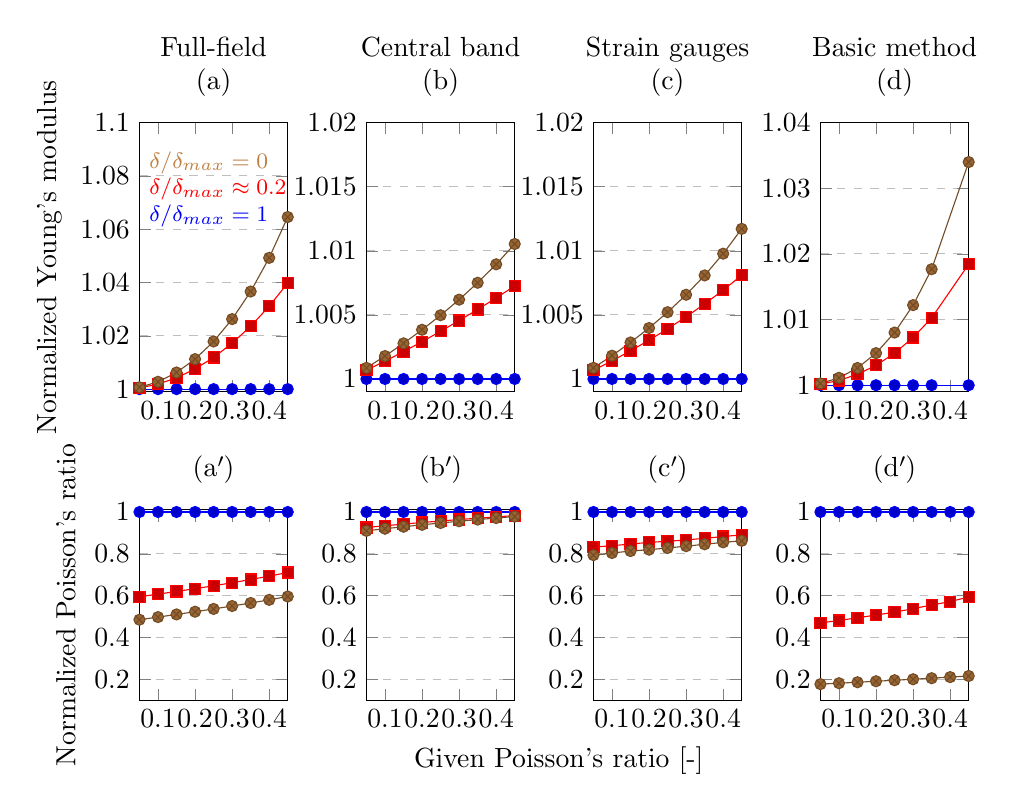
\begin{tikzpicture}[scale=1]

\pgfplotstableread{
nuxy	tr0	tr0.1	trINF
0.05	1	1.000678	1.000864
0.1	1	1.00139	1.00179
0.15	1	1.002135	1.002779
0.2	1	1.002912	1.003838
0.25	1	1.003719	1.004972
0.3	1	1.004556	1.00619
0.35	1	1.005424	1.007508
0.4	1	1.006323	1.008945
0.45	1	1.007256	1.010531

}\totarea

\pgfplotstableread{
nuxy	tr0	tr0.1	trINF	
0.05	1	1.00047	1.00068
0.1	1	1.00188	1.00275
0.15	1	1.00424	1.00625
0.2	1	1.00757	1.01126
0.25	1	1.01188	1.01788
0.3	1	1.01721	1.02627
0.35	1	1.02359	1.03663
0.4	1	1.0311	1.04926
0.45	1	1.03978	1.06458

}\chosenarea

\pgfplotstableread{
nuxy	tr0	tr0.1	trINF	
0.05	1	1.000683	1.000869
0.1	1	1.001413	1.001817
0.15	1	1.002193	1.00285
0.2	1	1.003024	1.003977
0.25	1	1.003908	1.005211
0.3	1	1.00485	1.006571
0.35	1	1.005855	1.00808
0.4	1	1.006931	1.009777
0.45	1	1.008091	1.011712



}\experiment


\pgfplotstableread{
nuxy	tr0	tr0.1	trINF	
0.05	1	1.00018	1.00027
0.1	1	1.00072	1.00113
0.15	1	1.00166	1.00263
0.2	1	1.00303	1.00489
0.25	1	1.00488	1.00802
0.3	1	1.00727	1.0122
0.35	1	1.01025	1.01767
0.45	1	1.01843	1.03399




}\experimentBasic

\pgfplotstableread{
nuxy	tr0	tr0.1	trINF	i0	i0.1	iINF
0.05	1	0.59508	0.48536	1	0.9382	0.8238
0.1	1	0.60748	0.49784	1	0.942	0.8349
0.15	1	0.62028	0.51052	1	0.946266667	0.846
0.2	1	0.63358	0.52349	1	0.951	0.8571
0.25	1	0.64744	0.53684	1	0.95616	0.86792
0.3	1	0.66198	0.55067	1	0.961866667	0.878266667
0.35	1	0.67731	0.56509	1	0.968228571	0.887942857
0.4	1	0.69357	0.58022	1	0.975575	0.89565
0.45	1	0.7109	0.5962	1	0.984644444	0.8698


}\nutotarea

\pgfplotstableread{
nuxy	tr0	tr0.1	trINF	i0	i0.1	iINF
0.05	1	0.926	0.91	1	0.9812	0.9456
0.1	1	0.9342	0.9201	1	0.9847	0.9552
0.15	1	0.9422	0.9296	1	0.988066667	0.964666667
0.2	1	0.94975	0.9387	1	0.99145	0.97405
0.25	1	0.95704	0.9474	1	0.99464	0.98336
0.3	1	0.963933333	0.9557	1	0.997766667	0.992733333
0.35	1	0.970542857	0.963628571	1	1.000742857	1.002171429
0.4	1	0.9768	0.971175	1	1.00355	1.011925
0.45	1	0.982755556	0.978377778	1	1.006288889	1.022933333

}\nuchosenarea

\pgfplotstableread{
nuxy	tr0	tr0.1	trINF	i0	i0.1	iINF
0.05	1	0.832	0.794	1	0.938	0.818
0.1	1	0.839	0.804	1	0.941	0.825
0.15	1	0.846666667	0.813333333	1	0.946666667	0.833333333
0.2	1	0.855	0.82	1	0.95	0.84
0.25	1	0.86	0.828	1	0.956	0.852
0.3	1	0.866666667	0.836666667	1	0.96	0.866666667
0.35	1	0.874285714	0.845714286	1	0.968571429	0.882857143
0.4	1	0.8825	0.855	1	0.975	0.905
0.45	1	0.891111111	0.862222222	1	0.984444444	0.931111111

}\nuexperiment


\pgfplotstableread{
nuxy	tr0	tr0.1	trINF	
0.05	1	0.469722892	0.177420121
0.1	1	0.481606855	0.181931174
0.15	1	0.494385965	0.186522064
0.2	1	0.507614213	0.191215676
0.25	1	0.521384929	0.196042474
0.3	1	0.537963909	0.200827288
0.35	1	0.555636789	0.205808631
0.4	1	0.571794872	0.211041361
0.45	1	0.593810666	0.216371772


}\nuexperimentBasic

%plot transv iso total area DSP

\begin{axis}[
name=b1,height=5cm,width=\textwidth/3.5,
    align =center,
    title={Full-field \\ (a)},
%    xlabel={Temperature [\textcelsius]},
    ylabel={Normalized Young's modulus},
    xmin=0.05, xmax=0.45,
    ymin=0.999, ymax=1.1,
        yticklabel style={/pgf/number format/fixed,
                  /pgf/number format/precision=3},
%     xtick={1,...,9},
%   ytick={0,20,40,60,80},
%      xticklabels={$0$,$1$,$.1$,$.2$,$.3$, $.4$, $6$,
%      $7$, $8$},
%     x tick label style={
%     rotate=60,anchor=east},
    ymajorgrids=true,
    grid style=dashed,
]
% \end{axis}    
% \begin{axis}[legend pos=outer north east]
 
 
    \addplot table[x=nuxy,y=tr0	] {\chosenarea}; \label{k1}
%     \addlegendentry{$\nu$=0.05}
    \addplot table[x=nuxy,y=tr0.1 ] {\chosenarea}; \label{k2}
%     \addlegendentry{$\nu$=0.1}
    \addplot table[x=nuxy,y=trINF ] {\chosenarea}; \label{k3}
%     \addlegendentry{$\nu$=0.15}


\node at (axis cs:0.05,1.085) [anchor=west,brown] {\footnotesize
{$\delta/\delta_{max}=0$}};
\node at (axis cs:0.05,1.075) [anchor=west,red] {\footnotesize
{$\delta/\delta_{max}\approx0.2$}};
\node at (axis cs:0.05,1.065) [anchor=west,blue] {\footnotesize
{$\delta/\delta_{max}=1$}};

\end{axis}


%plot transviso chosen area  DSP

\begin{axis}[legend pos=outer north east,
	name=b2,at={($(b1.east)+(1cm,0)$)},anchor=west, height=5cm,
	width=\textwidth/3.5,
	align =center,
	title={Central band\\(b)},
% xlabel={Poisson's ratio [-]},
%    ylabel={Measured stiffness [Pa]},
    xmin=0.05, xmax=0.45,
    ymin=0.999, ymax=1.02,
    yticklabel style={/pgf/number format/fixed,
                  /pgf/number format/precision=4},
%     xtick={1,...,9},
%    ytick={0,20,40,60,80},
%     xticklabels={$K=0$,$K=0.001$,$K=0.01$,$K=0.1$,$K=1$, $K=10$, $K=100$,
%     $K=1000$, $K=\infty$},
%     x tick label style={
%         rotate=60,anchor=east},
    ymajorgrids=true,
    grid style=dashed,
%     scaled y ticks=base 10:3,
    bar shift=0pt
]

    \addplot table[x=nuxy,y=tr0	] {\totarea}; \label{k1}
%     \addlegendentry{$\nu$=0.05}
    \addplot table[x=nuxy,y=tr0.1 ] {\totarea}; \label{k2}
%     \addlegendentry{$\nu$=0.1}
    \addplot table[x=nuxy,y=trINF ] {\totarea}; \label{k3}
%     \addlegendentry{$\nu$=0.15}

%Experimental approach

\end{axis}


\begin{axis}[legend pos=outer north east,
	name=b3,at={($(b2.east)+(1cm,0)$)},anchor=west,
	height=5cm,width=\textwidth/3.5, 	align =center,
	title={Strain gauges\\(c)},
%    xlabel={Temperature [\textcelsius]},
%    ylabel={Measured stiffness [Pa]},
    xmin=0.05, xmax=0.45,
    ymin=0.999, ymax=1.02,
    yticklabel style={/pgf/number format/fixed,
                  /pgf/number format/precision=3},
%     xtick={1,...,9},
%    ytick={0,20,40,60,80},
%     xticklabels={$K=0$,$K=0.001$,$K=0.01$,$K=0.1$,$K=1$, $K=10$, $K=100$,
%     $K=1000$, $K=\infty$},
%     x tick label style={
%         rotate=60,anchor=east},
    ymajorgrids=true,
    grid style=dashed,
    bar shift=0pt
]

    \addplot table[x=nuxy,y=tr0	] {\experiment}; \label{k1}
%     \addlegendentry{$\nu$=0.05}
    \addplot table[x=nuxy,y=tr0.1 ] {\experiment}; \label{k2}
%     \addlegendentry{$\nu$=0.1}
    \addplot table[x=nuxy,y=trINF ] {\experiment}; \label{k3}
%     \addlegendentry{$\nu$=0.15}




\end{axis}


\begin{axis}[legend pos=outer north east,
	name=b3a,at={($(b3.east)+(1cm,0)$)},anchor=west,
	height=5cm,width=\textwidth/3.5, 	align =center,
	title={Basic method\\(d)},,
%    xlabel={Temperature [\textcelsius]},
%    ylabel={Measured stiffness [Pa]},
    xmin=0.05, xmax=0.45,
    ymin=0.999, ymax=1.04,
    yticklabel style={/pgf/number format/fixed,
                  /pgf/number format/precision=3},
%     xtick={1,...,9},
%    ytick={0,20,40,60,80},
%     xticklabels={$K=0$,$K=0.001$,$K=0.01$,$K=0.1$,$K=1$, $K=10$, $K=100$,
%     $K=1000$, $K=\infty$},
%     x tick label style={
%         rotate=60,anchor=east},
    ymajorgrids=true,
    grid style=dashed,
    bar shift=0pt
]

    \addplot table[x=nuxy,y=tr0	] {\experimentBasic}; \label{k1}
%     \addlegendentry{$\nu$=0.05}
    \addplot table[x=nuxy,y=tr0.1 ] {\experimentBasic}; \label{k2}
%     \addlegendentry{$\nu$=0.1}
    \addplot table[x=nuxy,y=trINF ] {\experimentBasic}; \label{k3}
%     \addlegendentry{$\nu$=0.15}




\end{axis}

\begin{axis}
[name=b4,at={($(b2.south)-(0,1.5cm)$)},anchor=north,
height=4cm,width=\textwidth/3.5, title={(b\textprime)},
    xlabel={\hspace{3cm}Given Poisson's ratio [-]},
%     ylabel={Error Poisson's ratio},
    xmin=0.05, xmax=0.45,
    ymin=0.1, ymax=1.01,
        yticklabel style={/pgf/number format/fixed,
                  /pgf/number format/precision=3},
%     xtick={1,...,9},
%    ytick={0,20,40,60,80},
%     xticklabels={$K=0$,$K=0.001$,$K=0.01$,$K=0.1$,$K=1$, $K=10$, $K=100$,
%     $K=1000$, $K=\infty$}, 
%     x tick label style={
%     rotate=60,anchor=east},
    ymajorgrids=true,
    grid style=dashed,
]
% \end{axis}    
% \begin{axis}[legend pos=outer north east]
 
 
    \addplot table[x=nuxy,y=tr0	] {\nuchosenarea}; \label{nuk1}
%     \addlegendentry{$\nu$=0.05}
    \addplot table[x=nuxy,y=tr0.1 ] {\nuchosenarea}; \label{nuk2}
%     \addlegendentry{$\nu$=0.1}
    \addplot table[x=nuxy,y=trINF ] {\nuchosenarea}; \label{nuk3}
%     \addlegendentry{$\nu$=0.15}

\end{axis}


% plot transviso chosen area  DSP

\begin{axis}[
	name=b5,at={($(b1.south)-(0,1.5cm)$)},anchor=north, height=4cm,
	width=\textwidth/3.5, title={(a\textprime)},
%     xlabel={Given Poisson's ratio [-]},
   ylabel={Normalized Poisson's ratio},
    xmin=0.05, xmax=0.45,
    ymin=0.1, ymax=1.01,
%     yticklabel style={/pgf/number format/fixed,
%                   /pgf/number format/precision=3},
%     xtick={1,...,9},
%    ytick={0,20,40,60,80},
%     xticklabels={$0.05$,$0.3$,,,$0.45$},
%     x tick label style={
%         rotate=60,anchor=east},
    ymajorgrids=true,
    grid style=dashed,
    bar shift=0pt
]

    \addplot table[x=nuxy,y=tr0	] {\nutotarea}; \label{nuk1}
%     \addlegendentry{$\nu$=0.05}
    \addplot table[x=nuxy,y=tr0.1 ] {\nutotarea}; \label{nuk2}
%     \addlegendentry{$\nu$=0.1}
    \addplot table[x=nuxy,y=trINF ] {\nutotarea}; \label{nuk3}
%     \addlegendentry{$\nu$=0.15}

%Experimental approach

\end{axis}


\begin{axis}[name=b6,at={($(b3.south)-(0,1.5cm)$)},anchor=north,
height=4cm,width=\textwidth/3.5, title={(c\textprime)},
%    xlabel={Temperature [\textcelsius]},
%    ylabel={Measured stiffness [Pa]},
    xmin=0.05, xmax=0.45,
    ymin=0.1, ymax=1.01,
%     yticklabel style={/pgf/number format/fixed,
%                   /pgf/number format/precision=3},
%     xtick={1,...,9},
%    ytick={0,20,40,60,80},
%     xticklabels={$K=0$,$K=0.001$,$K=0.01$,$K=0.1$,$K=1$, $K=10$, $K=100$,
%     $K=1000$, $K=\infty$},
%     x tick label style={
%         rotate=60,anchor=east},
    ymajorgrids=true,
    grid style=dashed,
    bar shift=0pt
]

    \addplot table[x=nuxy,y=tr0	] {\nuexperiment}; \label{nuk1}
%     \addlegendentry{$\nu$=0.05}
    \addplot table[x=nuxy,y=tr0.1 ] {\nuexperiment}; \label{nuk2}
%     \addlegendentry{$\nu$=0.1}
    \addplot table[x=nuxy,y=trINF ] {\nuexperiment}; \label{nuk3}
%     \addlegendentry{$\nu$=0.15}




\end{axis}

\begin{axis}
[name=b6a,at={($(b3a.south)-(0,1.5cm)$)},anchor=north,
height=4cm,width=\textwidth/3.5, title={(d\textprime)},
%    xlabel={Temperature [\textcelsius]},
%    ylabel={Measured stiffness [Pa]},
    xmin=0.05, xmax=0.45,
    ymin=0.1, ymax=1.01,
%     yticklabel style={/pgf/number format/fixed,
%                   /pgf/number format/precision=3},
%     xtick={1,...,9},
%    ytick={0,20,40,60,80},
%     xticklabels={$K=0$,$K=0.001$,$K=0.01$,$K=0.1$,$K=1$, $K=10$, $K=100$,
%     $K=1000$, $K=\infty$},
%     x tick label style={
%         rotate=60,anchor=east},
    ymajorgrids=true,
    grid style=dashed,
    bar shift=0pt
]

    \addplot table[x=nuxy,y=tr0	] {\nuexperimentBasic}; \label{nuk1}
%     \addlegendentry{$\nu$=0.05}
    \addplot table[x=nuxy,y=tr0.1 ] {\nuexperimentBasic}; \label{nuk2}
%     \addlegendentry{$\nu$=0.1}
    \addplot table[x=nuxy,y=trINF ] {\nuexperimentBasic}; \label{nuk3}
%     \addlegendentry{$\nu$=0.15}




\end{axis}


\end{tikzpicture}

\caption{Normalized Young's moduli and Poisson's ratio vs. given Poisson's ratio
of transversely isotropic material with different slippage conditions relative
to different ways of measuring strain}
\label{fig:strainmethods}


\end{figure}
\end{center}



% 
% Three plots can be compared in Figure \ref{fig:isovstriso}. 
% From the plots a)-c) one can compare the difference between the measured and actual 
% Young's moduli depending on the Poisson's ratio versus the
% displacement of the top edge. The displacement is represented as a displacement
% factor which is relation between the actual $\delta$ and maximum
% displacement $\delta_{max}$ that is based on factor $K$. For all simulations the
% barrelling is leading to an overestimation of the Young's moduli. This is caused by the strain field in the area close to the edges, where constrained material has a stiffer response.
% In general, for increasing Poisson's ratio, the error becomes larger. 
% For the transversely isotropic material in Figure
% \ref{fig:isovstriso} $b,c$ the error in Young's moduli is less in
% transverse direction $T$ than in the axial direction $L$.
% This difference in behaviour can be discussed by examining the strain fields for isotropic and 
% transversely isotropic materials shown in of Figure
% \ref{fig:Error} a, b and c. One can
% observe the cones of the constraining effect that are originating from the top
% and bottom. The constraining effect is dominant on the $25\%$ of height
% from the horizontal edges of the model. Whereas in transversely isotropic
% material in the $TT$ plane , the is spread less in the surface area.\\
% Observation of Poisson's ratio values showed the opposite behaviour concerning
% the measurement.
% Figure \ref{fig:isovstriso} $a'$ showed that the relative error for the
% Poisson's ratio is less significant in isotropic material. This is supported
% with the corresponding strain field in Figure \ref{fig:Error} $a'$. The normal
% Poisson's ratio values are within the central area of the model. 
% Alternatively Figure \ref{fig:isovstriso} $b'$ and $c'$ describing the effect
% of barrelling on the measured materials Poisson's ratio in transversely isotropic material. 
% It is seen that for the $LT$ planes the constraining effect influence the
% measurements significantly. For example, for the displacement factor $\delta/\delta_{max}\approx0.2 $ where $K=0.1$,  the Poisson's ratio is
% underestimated by $30-40\%$.
% The same situation is for the plane $TT$ but the effect is less severe.
% Referring to Figure \ref{fig:Error} $a-c$  we can see that the constraining effect is
% crucial for the estimation of the Poisson's ratio. Blue coloured area where the error is above $5\%$ spreading from the horizontal edges of 
% the model throughout the central area of the material. So the most accurate
% estimation of Poisson's ratio is in the central area close to the vertical
% edges of the cube as it seen in Figure \ref{fig:Error} $c,d$. However it was
% mentioned that usage of strain gauges are usually placed in the center of the
% sample, whereas presented results are supporting the fact that central
% region of the sample is not always beneficial for the measurements. In this
% case the usage of DSP is preferable. 
% 
% 
% \begin{description}
% \item{\textit{Strain measurement}}
% \end{description}
% Measured mechanical properties varies with strain measurement methods. In
% present work, three methods were measured and compared. The
% first method is shown in Figure \ref{fig:strainmethods}$b$, where the total area
% including the constrained region is taken for measuring the strain.  
% Here the error originates from the underestimated axial strains that are the
% reason of constraining effect of horizontal edges. However the evaluation of
% Poisson's ratio has less error due to inclusion of the total area into the
% strain evaluations. Strain field in Figure \ref{fig:Error}$b$ shows that total
% area has more regions where error is not significant.

In the second approach only the middle 60\% of the area part was
taken for determination of strain. The plot in Figure
\ref{fig:strainmethods}(a) shows that with this method the Young's moduli is
less overestimated than in the first approach.\par In the third approach where
the Standard ASTM-D143-94 with strain gauge technique was used, the error is very close to the one in
second approach. The plot in Figure \ref{fig:strainmethods}(c) depicts that
this happens because the strain is measured between two points in the center of 
the sample where the constraining effect is less severe. 

Large error values for the Young's
modulus close to the horizontal edges of isotropic model are clearly visible in
Figure \ref{fig:Error}(a). The opposite is true for the transversely isotropic
sample in Figure \ref{fig:Error}(b,c), for $LT$ plane 
the Young's moduli in the central area is overestimated whereas for $TT$ plane
the strain field looks similar to the isotropic material.\par
These simulations are supporting the experimental results in Figure
\ref{fig:explot}. Where the average strain diagram for the total area is showing larger Young's moduli than
the one for the chosen area.
Additional outcomes are deduced  while observing the error fields in Figure
\ref{fig:Error}(a\textprime-c\textprime). The ASTM-D143-94 standard
\cite{american2009standard} requires installation of strain gauges in the center of the sample. This approach will
lead to underestimation of Poisson's ratio in transversely isotropic cubic
sample due to the barrelling formation. On the other hand accurate values will
be obtained for the isotropic material, where the constraining effect influence
the horizontal edges of the sample. The chosen central area of the isotropic
sample is most favourable for accurate measurements.


\begin{description}
\item{\textit{Barrelling in orthotropic material}}
\end{description}
As it was mentioned, the barrelling is more severe in the isotropic material and
less in transverse isotropic. To check whether this stands for the orthotropic
materials, a true orthotropic model was simulated, based on wood material properties
that were experimentally determined \cite{vorobyevcharacterisation}.

\begin{center}% note that \centering uses less vspace...
\begin{figure}[h]
\pgfplotsset{every axis legend/.append style={
		at={(0.5,1.03)},
		anchor=north}}

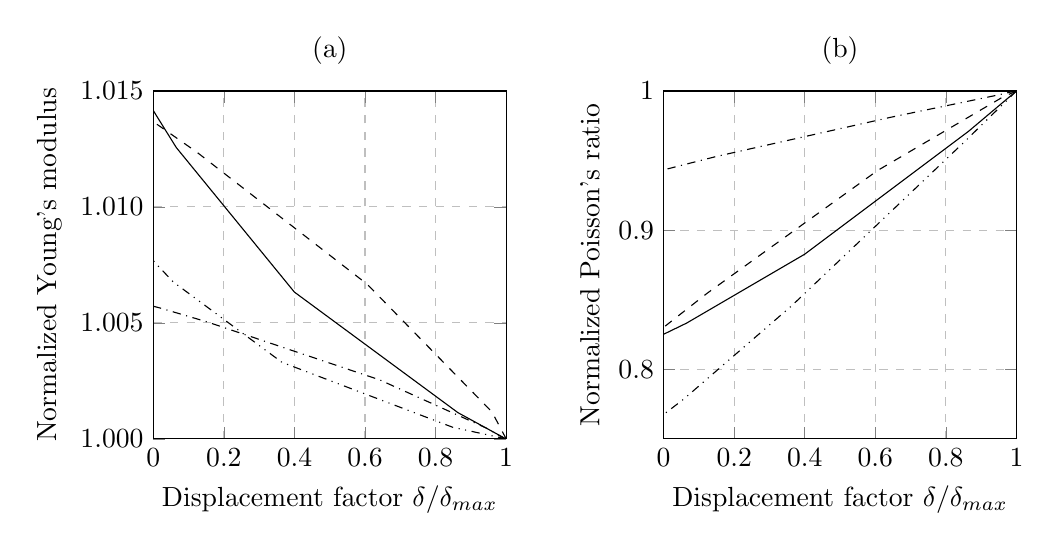
\begin{tikzpicture}[scale=1]

	\pgfplotstableread{
K	ZY	dZY	ZX	dZX	XZ	dXZ	XY	dXY
0	1	0.99931	1	1	1	1	1	0.99666
0.001	1.00113	0.86336	1.00116	0.95989	1.0005	0.84846	1.00045	0.94592
0.01	1.00633	0.39972	1.00667	0.60587	1.0033	0.36457	1.00254	6.42E-01
0.1	1.01256	0.06514	1.01236	0.12346	1.00677	0.05606	1.00505	1.51E-01
1	1.01398	0.00698	1.01353	0.01348	1.00759	0.0055	1.00565	1.74E-02
10	1.01414	0.000703066	1.01365	0.00103	1.00768	0.000058874	1.00571	0.00177
100	1.01416	7.03579E-05	1.01367	-0.000226463	1.00769	-0.000489077	1.00572	0.000176984
1000	1.01416	7.0363E-06	1.01367	-0.000352727	1.00769	-0.000543916	1.00572	1.77012E-05


}\datatable

\pgfplotstableread{
K	ZY	dZY	ZX	dZX	XZ	dXZ	XY	dXY
0	1	1	0.99999	1	0.99996	1	0.99996	0.99666
0.001	0.97083	0.86336	0.99543	0.95989	0.96247	0.84846	9.97E-01	0.94592
0.01	0.88268	0.39972	0.94277	0.60587	0.84601	0.36457	9.81E-01	0.64214
0.1	0.83318	0.06514	0.85465	0.12346	0.77836	0.05606	9.53E-01	0.15068
1	0.82602	0.00698	0.83283	0.01348	0.7686	0.0055	0.9444	0.0174
10	0.82528	0.000703066	0.8303	0.00103	0.76759	0.000058874	0.94339	0.00177
100	0.8252	7.03579E-05	0.83005	-0.000226463	0.76749	-0.000489077	0.94328	0.000176984
1000	0.82519	7.0363E-06	0.83002	-0.000352727	0.76748	-0.000543916	0.94327	1.77012E-05



}\datatableA




\begin{axis}[
name=plot0,height=6cm,width=\textwidth/2,
    title={(a)},
	xlabel={Displacement factor $\delta/\delta_{max}$},
    ylabel={Normalized Young's modulus},
    xmin=0, xmax=1,
    ymin=1, ymax=1.015,
%     xtick={1,...,9},
%     xticklabels={$0$,$0.001$,$0.01$,$0.1$,$1$, $10$, $100$,
%     $1000$, $\infty$}, 
%         x tick label style={yshift=-1ex,
%         rotate=45,anchor=east		},
    y tick label style={
        /pgf/number format/.cd,
            fixed,
            fixed zerofill,
            precision=3,
        /tikz/.cd},
%     ytick={0,1.01,1.015,1.02,1.025},
    ymajorgrids=true,
    xmajorgrids=true,
    grid style=dashed,
]
% \end{axis}    
% \begin{axis}[legend pos=outer north east]
 
 
    \addplot+[solid, black, mark=] table[x=dZY,y=ZY] {\datatable};
%     \addlegendentry{$\nu$=0.05}
    \addplot+[dashed, black, mark=] table[x=dZX,y=ZX] {\datatable};
%     \addlegendentry{$\nu$=0.1}
    \addplot+[dashdotdotted, black, mark=] table[x=dXZ,y=XZ] {\datatable};
%     \addlegendentry{$\nu$=0.15}
    \addplot+[dashdotted, black, mark=] table[x=dXY,y=XY] {\datatable};

\end{axis}

\begin{axis}[
name=plot1,at={($(plot0.east)+(2cm,0)$)},anchor=west,
height=6cm,width=\textwidth/2, title={(b)},
	xlabel={Displacement factor $\delta/\delta_{max}$},
    ylabel={Normalized Poisson's ratio},
    xmin=0, xmax=1,
    ymin=0.75, ymax=1,
    yticklabel style={/pgf/number format/fixed,
                  /pgf/number format/precision=3},
%     xtick={1,...,9},
%    ytick={0,20,40,60,80},
%     xticklabels={$0$,$0.001$,$0.01$,$0.1$,$1$, $10$, $100$,
%     $1000$, $\infty$},
%             x tick label style={yshift=-1ex,
%         rotate=45,anchor=east		}, 
    ymajorgrids=true,
    xmajorgrids=true,
    grid style=dashed,
    bar shift=0pt
]

    \addplot+[solid, black, mark=] table[x=dZY,y=ZY] {\datatableA};
    \label{VasaZY}
%     \addlegendentry{$\nu$=0.05}
    \addplot+[dashed, black, mark=] table[x=dZX,y=ZX]
    {\datatableA};
    \label{VasaZX}
%     \addlegendentry{$\nu$=0.1}
    \addplot+[dashdotdotted, black, mark=] table[x=dXZ,y=XZ] {\datatableA};
    \label{VasaXZ}
%     \addlegendentry{$\nu$=0.15}
    \addplot+[dashdotted, black, mark=] table[x=dXY,y=XY] {\datatableA};
    \label{VasaXY}



\end{axis}


\end{tikzpicture}


\captionsetup{justification=centering}
\caption{Simulated and normalized results based on experiment of
orthotropic material. a) Young's moduli and b) Poisson's ratio while measuring
chosen strain field from directions LT(\ref{VasaZY}),
LR(\ref{VasaZX}), 
TL(\ref{VasaXZ}), 
TR(\ref{VasaXY}).}


\label{fig:ortho}
\end{figure}

\end{center}

The results is for normalised Young's moduli in all wood orthotropic directions
and Poisson's ratio versus the displacement factor are plotted in Figure
\ref{fig:ortho}. The notation for the wood planes in Figure is corresponding to
the wood principal orthotropic directions, where Longitudinal (L), Radial (R),
Tangential (T). \par It shows that the magnitude of error is less than those for
the transversely isotropic material.
In case of identifying the Young's moduli $E_{\mathrm{L}}$, plane  LT might be
beneficial. This is due to the less slope of LT curve in comparison to LR in
Figure \ref{fig:ortho}a. \par
As for transversely isotropic material the Poisson's ratio is underestimated
with the increasing constraining effect the same is observed for the orthotropic
material simulation. The magnitude of error is spread, however the
$\nu_{\mathrm{LT}}$, $\nu_{\mathrm{LR}}$, $\nu_{\mathrm{TR}}$ are less
influenced by the barrelling. Contrary $\nu_{\mathrm{TL}}$ is more
underestimated than the others, presented in Figure \ref{fig:ortho}b. When L
direction is in transverse plane, the geometrical response is less significant
because of its stiffness. Therefore the magnitude of possible error depending on
barrelling is larger. However having the $\nu_{\mathrm{LT}}$,
$\nu_{\mathrm{LR}}$, $\nu_{\mathrm{TR}}$ ratios the symmetry principle can
be used to determine the rest.










\section{Conclusions}

The barrelling in cubic samples subjected to compressive testing is an phenonomenon that can influence the
estimation of the engineering elastic constants. The magnitude of the error depends on the type of material anisotropy, viz. 
isotropic, transversely isotropic and orthotropic materials, which are representative of most load carrying materials :

\begin{itemize}
  \item \textit{Isotropic} material is affected by the barrelling the most.
  As an example, the measured Young's moduli is overestimated  by up to 20\%  for 
  materials with a Poisson's ratio of $\nu=0.45$. The estimation of Poisson's ratio
  gives less errors in comparison to other materials.
  \item \textit{Transversely-isotropic} material shows an overestimation of Young's 
  moduli in both the L and T 
  directions but less in comparison with the isotropic material. The error is larger for the LT  and TT plane in the estimation of the Poisson's ratio. 
  \item \textit{Orthotropic} material was simulated using the experimental 
  input data for the experimentally characterised archaeological wood. 
  The result shows an overestimation of Young's moduli in all principal planes 
  of orthotropic wood, but the error is similar to that of the TT plane in 
  transversely-isotropic material, which is below $1.5\%$ of error margin.
\end{itemize}

The strain measurement methods showed advantages of using a central band for
the estimation of strains in the corresponding plane. The results can be 
summarized as follows:

\begin{itemize}
  \item Using the entire strain field from the \textit{full field} measurement of the sample plane
  is leading to relative large errors in the estimated elastic properties, since
  the constrained regions close to the platens form a large part of the 
  strain measurement.  In the severe case of rubber-like, almost incompressible 
  materials with $\nu=0.45$, the measured Young's moduli is overestimated by up 
  to a distressing level of 20 \% . On the other hand, the estimation of Poisson's 
  ratio gives smaller errors comparable to the transverse isotropic and orthotropic 
  materials.
  \item Strains from the \textit{strain gauge} measurement 
  (representing the strandaridized metod) shows smaller errors in the 
  estimated elastic properties than for the full-field approach. 
  However, the measurements are done between the two points and inside the 
  constraining cone emanating from the friction of the platens. 
  Thus, the strain gauge method leads to non-negligible errors as well.
  \item  The \textit{central band} of full strain field in the centre of the 
  sample was chosen to cover a zone which is relatively unperturbed by the 
  frictional platens in the compressive test. Here, relatively good results with 
  limited errors were obtained.
\end{itemize}

Two strain-field measuring techniques, \textit{full field} 
and \textit{central band}
were used in the experiments. The elastic properties were estimated from the 
strain measurements in the central band only, as this was shown to be more accurate. 
Since full-field measurement techniques are becoming more commonplace in mechanical 
testing laboratories, their advantages to point or line measurements 
(e.g. strain gauges or extensometers) should be exploited. 
It is recommended to use the part of the strain field that is only moderately 
affected by loading constraints from the test rig. In the case of compressive 
testing of cubes, a suitable part has been found to be a central lateral band 
covering 60\% of the observed face. 




\section*{Acknowledgements}
The work presented in this article has been performed in collaboration with the National Maritime Museums of Sweden
and, in particular, the Vasa Museum. The work has been carried
out within the ``Support Vasa'' project, where financial contributions come from the funding agencies  Formas, Vinnova and
Vetenskapsr{\aa}det in addition to the National Martime Museums of Sweden and Uppsala University. 
\section*{References}
\bibliography{mybibfile}



\pagebreak
\section*{Tables}

\begin{description}

\item[]
\begin{table}[!htbp]\
\caption{Engineering elastic constants used in the model} % title of Table
\centering % used for centering table
\begin{tabular}{c c c c c c c c c} % centered columns (4 columns)
\hline\hline %inserts double horizontal lines
 $E_{\mathrm{T}}$ (GPa) & $E_{\mathrm{T}}$ (GPa) & $E_{\mathrm{L}}$ (GPa) &
 $G_{\mathrm{LT}}$ (GPa) & $G_{\mathrm{TT}}$ (GPa) & $G_{\mathrm{LT}}$ (GPa) &
$\nu_{\mathrm{TL}}$ & $\nu_{\mathrm{TT}}$ & $\nu_{\mathrm{TL}}$ \\ % inserts
% table heading

\hline % inserts single horizontal line
$E$ & $E$ & $a{E}$ & $\frac{\Big(b\big[a-1\big]+1\Big){E}}{2(1+\nu)}$  &
$\frac{a{E}}{2(1+\nu)}$ & $\frac{\Big(b\big[a-1\big]+1\Big){E}}{2(1+\nu)}$ & $\frac{\nu}{a}$ & $\nu$ & $\frac{\nu}{a}$ \\
% inserting body of the table
[1ex] % [1ex] adds vertical space
\hline %inserts single lines

\multicolumn{6}{l}{%
  \begin{minipage}{9cm}%
\footnotesize Note: $E=1$; $\nu=0.25$; Parameter $a=1$ for isotropic and $a=10$
    for transversely isotropic material model; Shear stiffness parameter 
    $b=1$ for isotropic and for transversely isotropic
    $b=2$.
      \end{minipage}%
}\\
      
	
\end{tabular}

\label{table:simulpar} % is used to refer this table in the text
\end{table}

\item[]
\begin{table}[!htbp]\
\caption{Typical engineering properties of transversely isotropic materials} % title of Table
\centering % used for centering table
\begin{tabular}{l c c c c } % centered columns (4 columns)
\hline\hline %inserts double horizontal lines

& \begin{tabular}{@{}c@{}}
Vasa oak \\
(ref. nr. 65742)  \cite{vorobyevcharacterisation} \end{tabular} &
\begin{tabular}{@{}c@{}}Graphite-polymer \\ composite \cite{hyer2009stress} \end{tabular} & \begin{tabular}{@{}c@{}}Glass-polymer \\
composite \cite{hyer2009stress}\end{tabular}  & \begin{tabular}{@{}c@{}}
 S2 glass reinforced  \\
epoxy \cite{american2002composite} \end{tabular}  
\\
%  & $E_{1}$  & $E_{2}$ (GPa) & $E_L$ (GPa) & $\nu_{12}$ & $\nu_{13}$
% & $\nu_{23}$ & $G_{12}$ (GPa) & $G_{13}$ (GPa) & $G_{23}$ (GPa) \\ % inserts
% % table heading

\hline % inserts single horizontal line

$E_{\mathrm{T_1}}$ (GPa) & 0.60 & 12.10 & 15.20 & 14.7\\
$E_{\mathrm{T_2}}$ (GPa) & 0.35 & 12.10 & 15.20 & 14.7\\
$E_{\mathrm{L}}$ (GPa) & 6.75 & 155.0 & 50.00 & 49.3\\

$G_{\mathrm{LT_2}}$ (GPa) & 0.62 & 4.40 & 4.70 & 6.8\\
$G_{\mathrm{T_1T_2}}$ (GPa) & 0.14 & 3.20 & 3.28 & 4.9\\
$G_{\mathrm{LT_1}}$ (GPa) & 0.33 & 4.40 & 4.70 & 6.8\\

$\nu_{\mathrm{LT_1}}$ (-) & 0.37 & 0.248 & 0.254 & 0.296\\
$\nu_{\mathrm{T_1T_2}}$ (-) & 0.30 & 0.458 & 0.428 & 0.449\\
$\nu_{\mathrm{LT_2}}$ (-) & 0.69 & 0.248 & 0.254 & 0.306\\





% Graphite-polymer composite & 12.10 &  & 12.10 & 155.0 & 0.458 & 0.248 & 0.248 &
% 0.6 & 0.72 & 0.72\\
% % inserting body of the table
% Transverse isotropic & 1.49 & $E_1=E_2$ & 12.14 & 0.66 & 0.06 & 0.04 & 0.2 &
%  0.6 & 0.72\\
% Isotropic & - & - & 12.14 \\
\hline %inserts single line
\end{tabular}
\label{table:nonlin} % is used to refer this table in the text
\end{table}
\end{description}


%%%%%%%%%%% VIDEO CAPTIONS

%% If submitting video's as a supplement to the manuscript, include only the video captions here (not the figures).  Videos are uploaded separately in the online Elsevier Editorial Submission process.  If videos are not included, comment out this section.

%% Do not remove the page break here.
\pagebreak


\end{document}
